\documentclass[12pt,a4paper]{article}
\usepackage[utf8]{inputenc}
\usepackage[german]{babel}
\usepackage[T1]{fontenc}
\usepackage{amsmath}
\usepackage{amsfonts}
\usepackage{amssymb}
\usepackage{graphicx}
\usepackage[left=2.5cm,right=2.5cm,top=2cm,bottom=2cm]{geometry}
\author{Gruppe C14 \\ Julián Häck, Martin Koytek, Lars Wenning, Erik Zimmermann}
\usepackage{float}
\begin{document}
\section{Bestimmung der Schallgeschwindigkeit durch Laufzeitmessung}
\subsection{Versuchsbeschreibung}
%Kurze Darstellung der physikalischen Grundlagen und Ziele der Versuche, %die zum Verständnis
%des Versuches/Protokolls benötigt werden. (max. 1 Seite)
Bei der Bestimmung der Schallgeschwindigkeit in Luft durch eine Laufzeitmessung wird eine Störung in verschiedenen Abständen aufgezeichnet, um anschließend den Abstand gegen die vom Schall benötigte Zeit zum Zurücklegen dieser Strecke aufgetragen. Aus der Steigung der durch die Messwerte gefitteten Geraden ergibt sich somit die Schallgeschwindigkeit:
\begin{equation}
v=\frac{s}{t}
\end{equation}
Für die Temperaturabhängigkeit gilt:
\begin{equation}
v=v_0\cdot \sqrt{\frac{T}{T_0}} \label{Temperaturabhängigkeit}
\end{equation} 
\subsection{Versuchsaufbau und Durchführung}
%Genaue Beschreibung der verwendeten Aufbauten unter Verwendung von Skizzen oder Photos
%Beschreibung der Messwerterfassungseinstellungen (eingestellte Messzeiten, Messbedingungen,
%Trigger, Anzahl der Messungen) und der Durchführung der Versuche. (max. 1 Seite)
\begin{figure}[H]
\centering
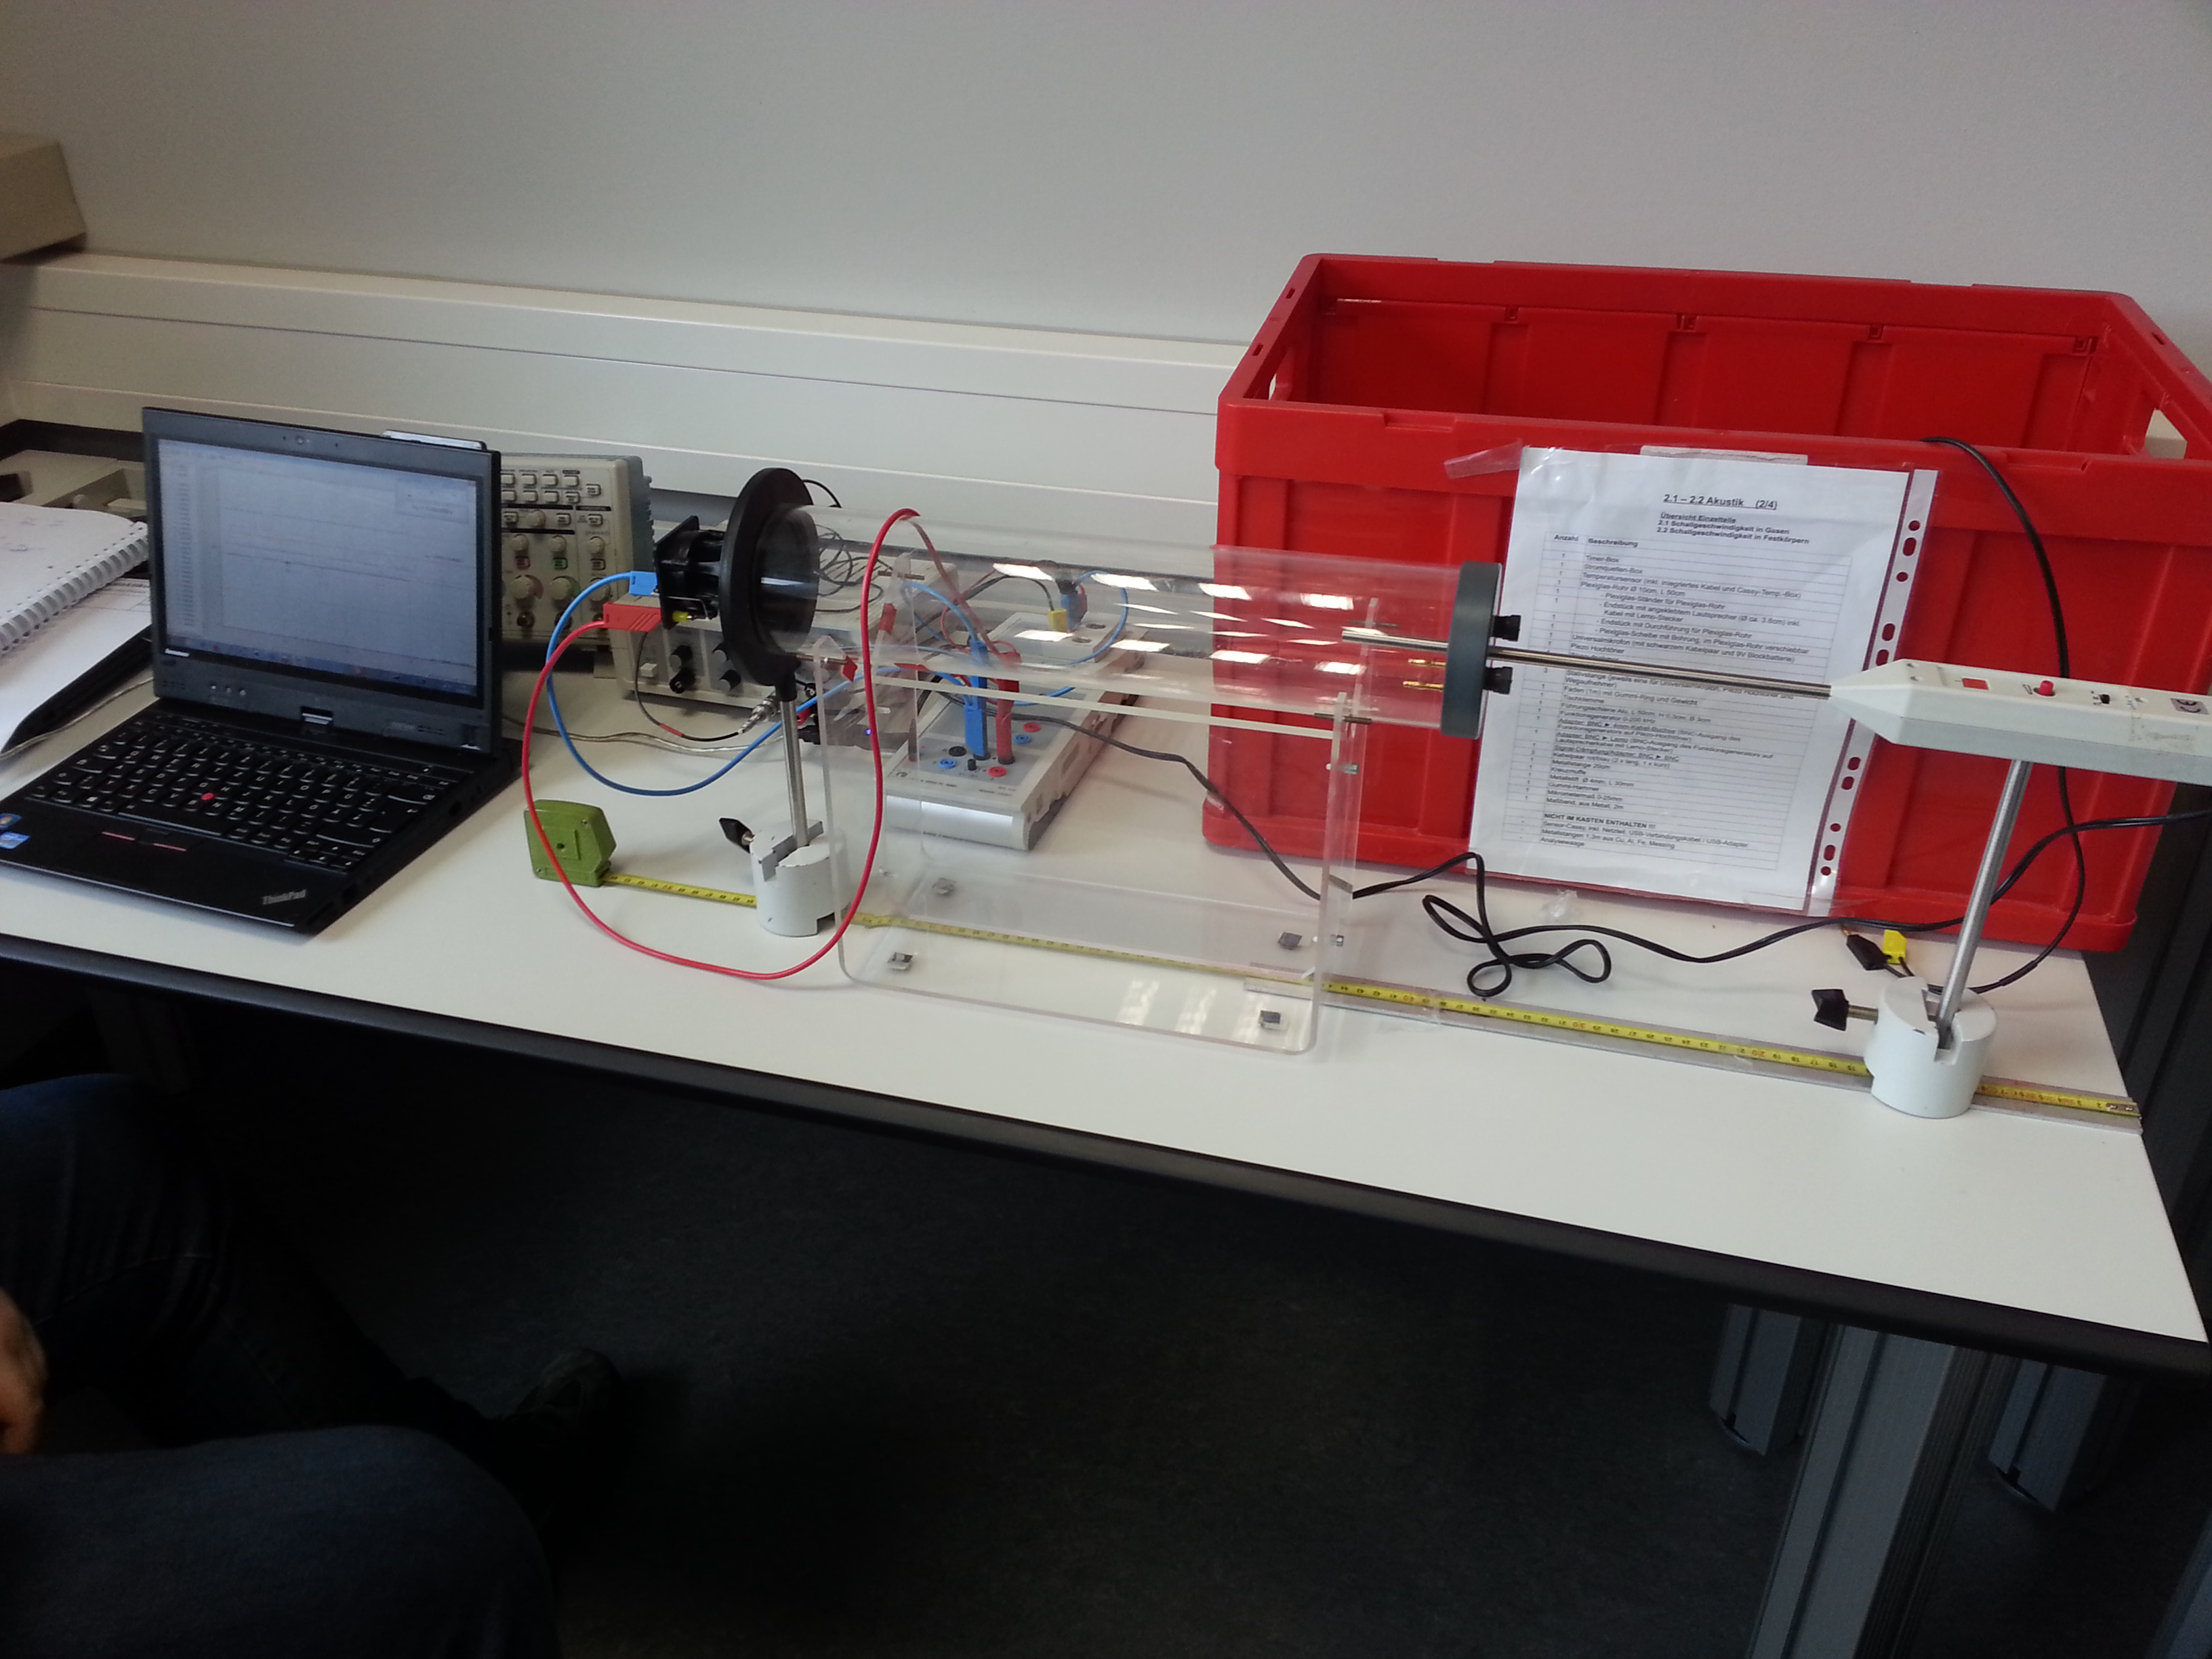
\includegraphics[scale=0.15]{Bilder/laufzeit-cassy.jpg}
\caption{Versuchsaufbau der Laufzeitmessung mit dem Sensor-Cassy.}
\end{figure}
\begin{figure}[H]
\centering
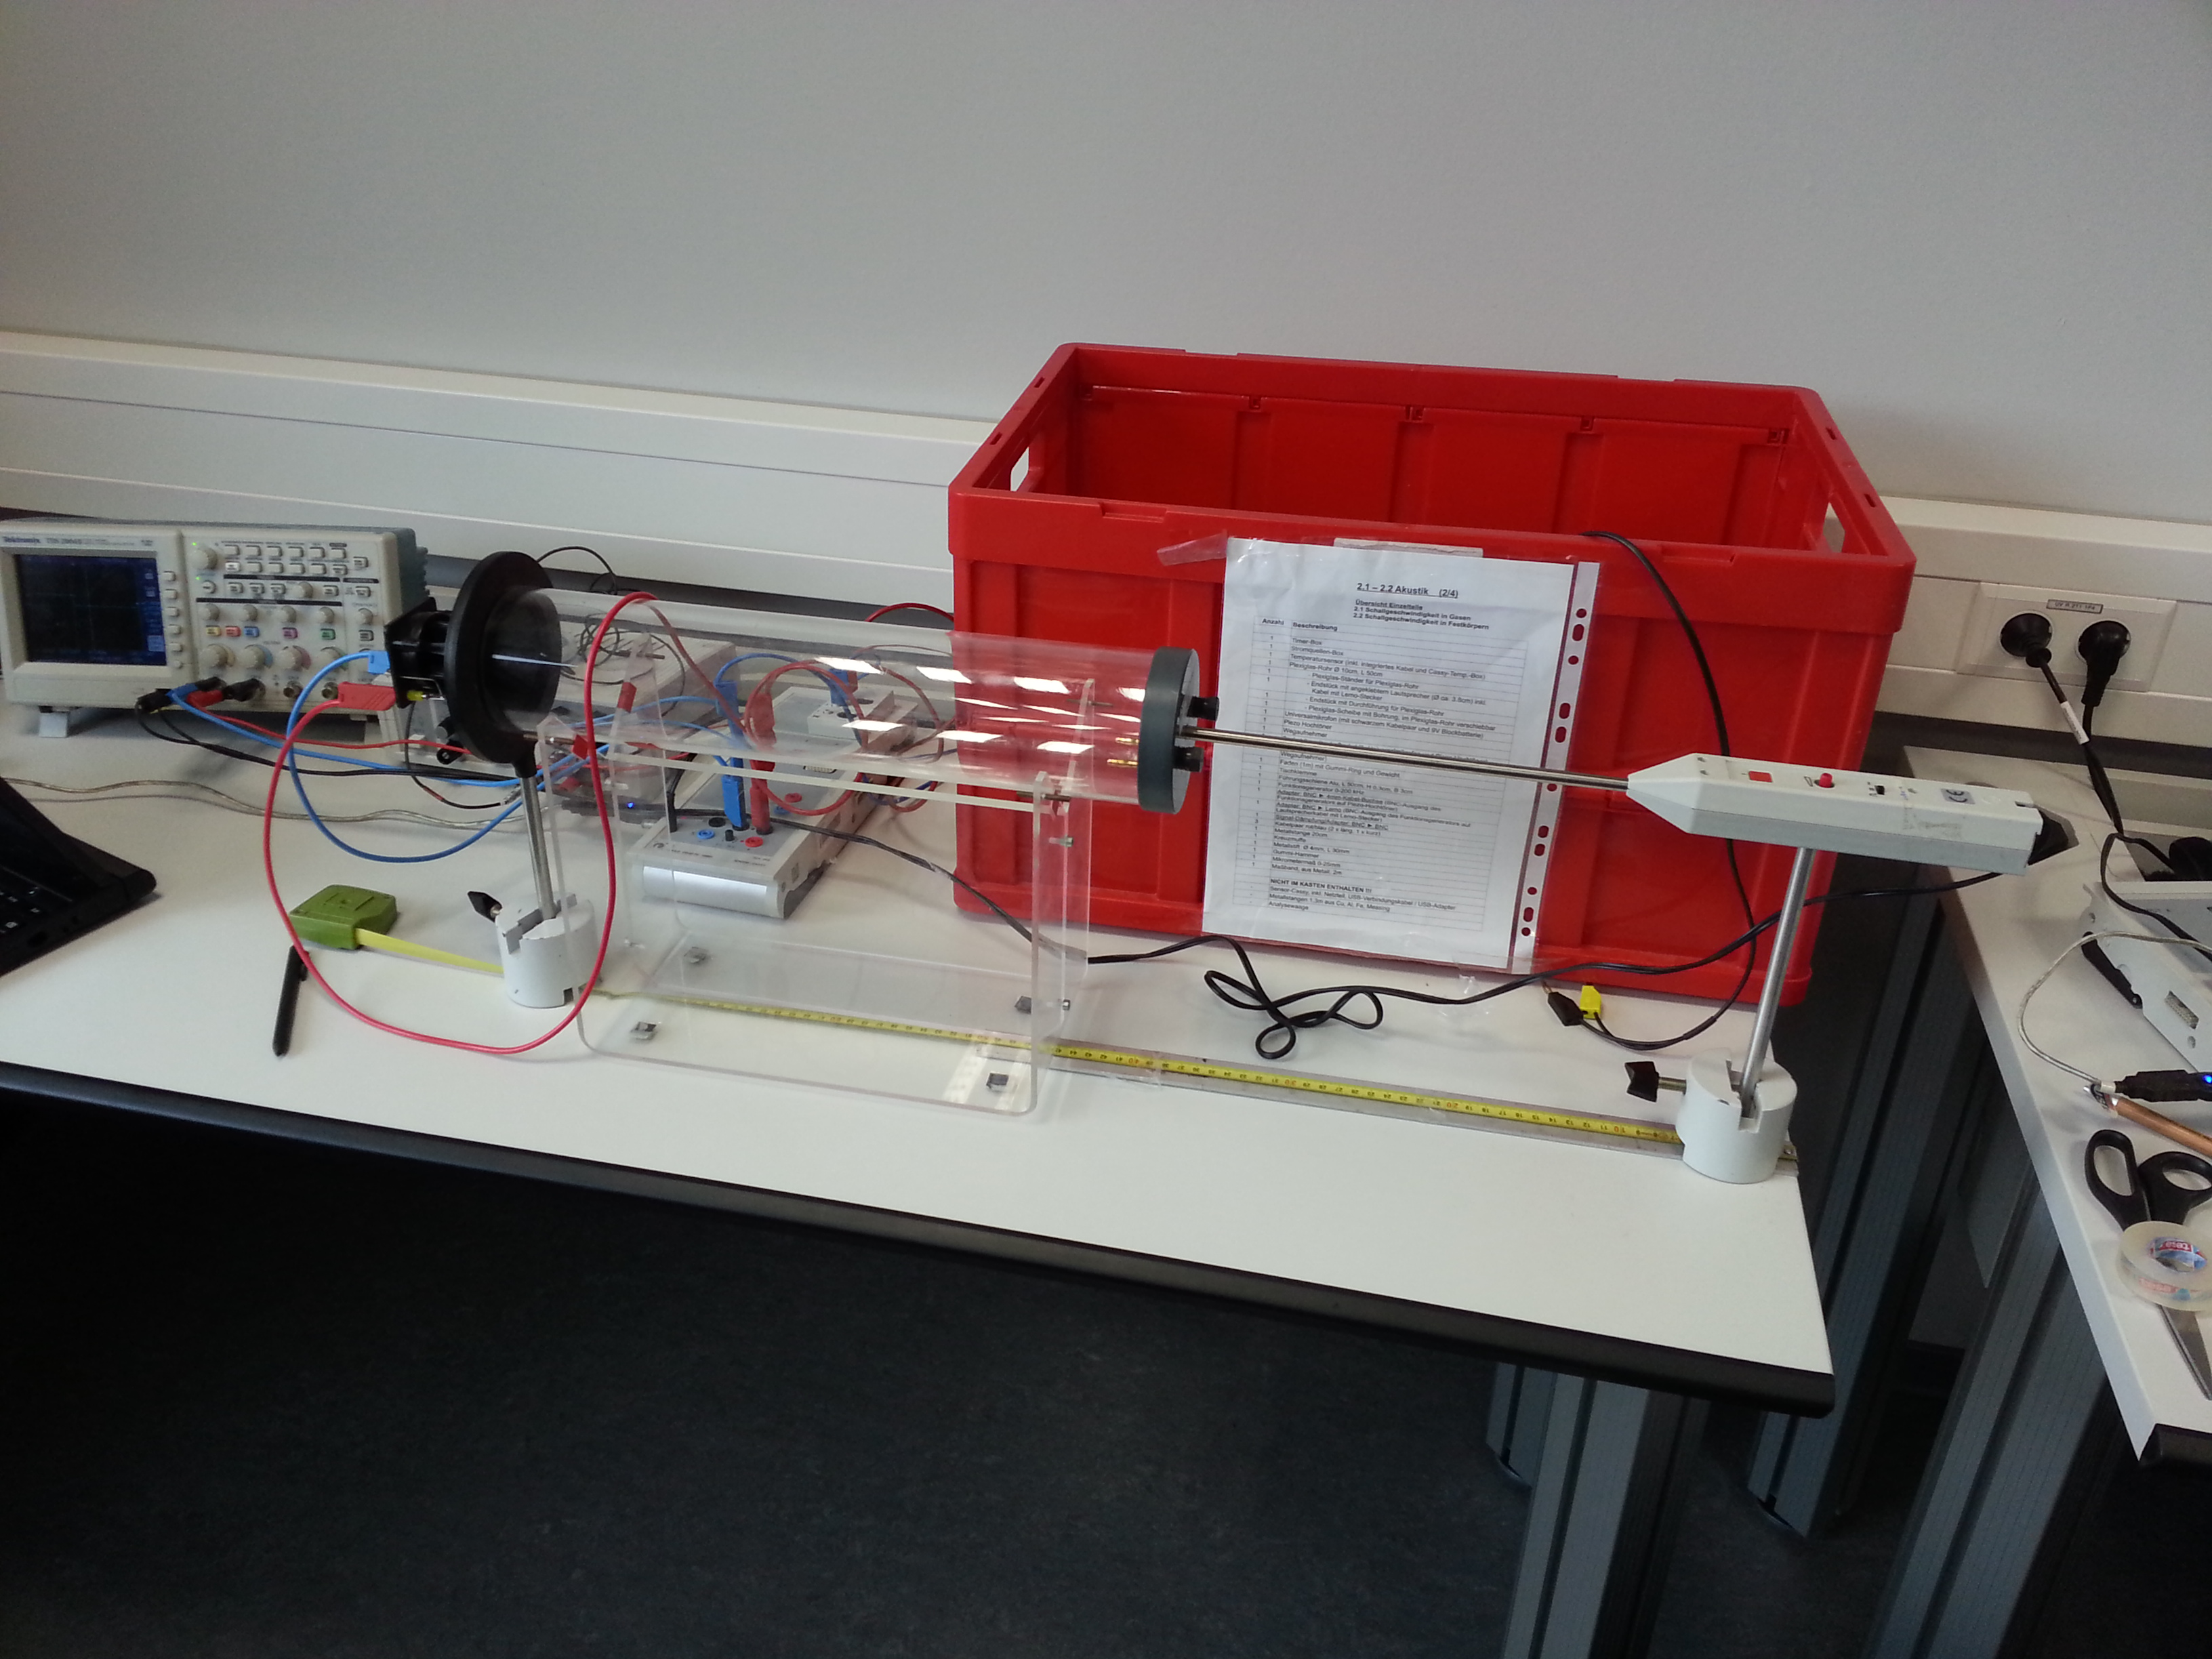
\includegraphics[scale=0.15]{Bilder/laufzeit-oszi.jpg}
\caption{Versuchsaufbau der Laufzeitmessung mit dem Oszilloskop.}
\end{figure}


Bei dem Versuch wurde mit einem Piezo-Hochtöner am einen Ende eines Schallrohrs eine Störung erzeugt, die dann in verschiedenen Abständen innerhalb des Schallrohrs von einem Mikrofon im Trigger-Modus aufgezeichnet wurde. Der Piezo-Hochtöner wurde sowohl an eine Timerbox, die an das Sensor-Cassy anschlossen wurde, als auch parallel dazu an das Relais des Sensor-Cassys angeschlossen. Das Mikrofon wurde ebenfalls an die Timerbox angeschlossen. Beim Start der Messung wird das Relais geschlossen, wodurch das Piezoelement entladen wird und die Störung aussendet. Nach Schließen des Relais wird dieses wieder aufgeladen. Beim  Eintreffen der Störung am Mikrofon, liefert dieses das Stopp-Signal für die Zeitmessung.
Anschließend wurde dieser Versuch noch einmal mit einem Oszilloskop aufgezeichnet und der Abstand der Spannungspeaks mit Hilfe des Cursors abgelesen.
Außerdem wurde während des Versuchs die Temperatur der Luft gemessen.
\newpage
\subsection{Versuchsauswertung}
\subsubsection{Rohdaten}
\begin{figure}[H]
\centering
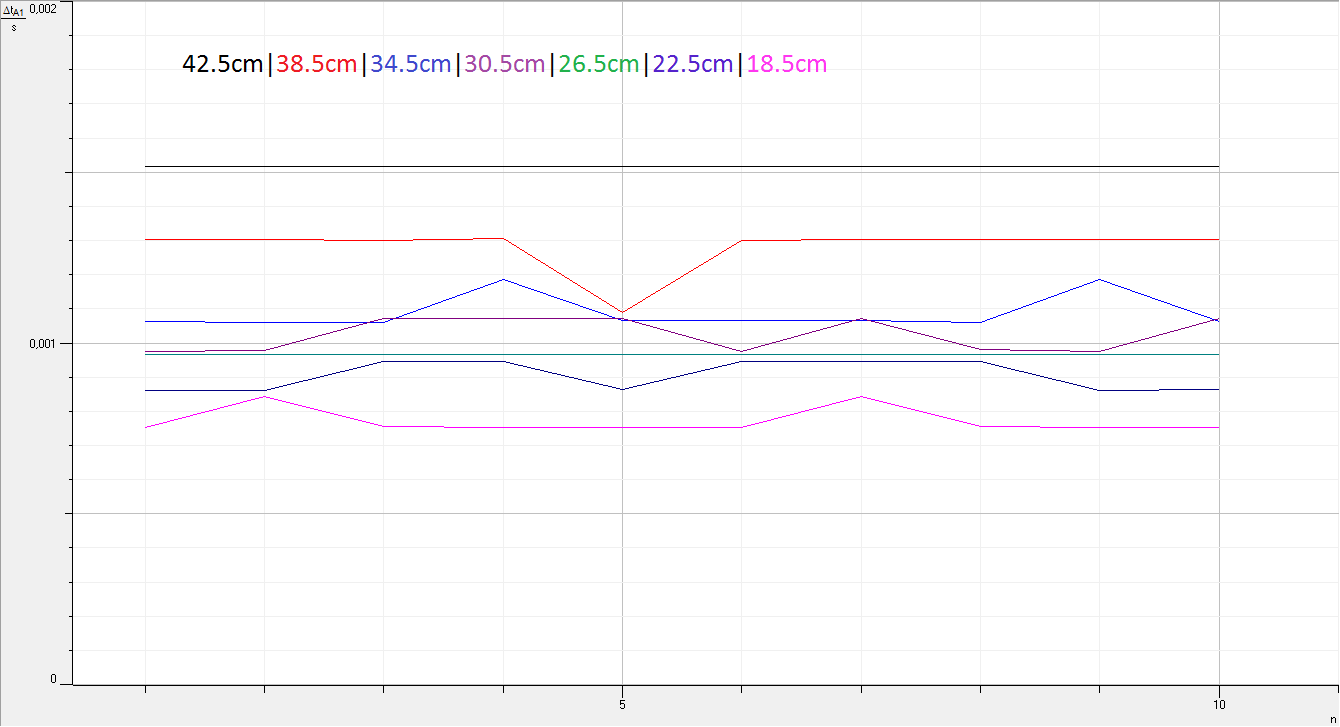
\includegraphics[scale=0.6]{Bilder/Rohdaten-Laufzeitmessung.png}
\caption{Beispiel einer Laufzeitmessung mit dem Sensor-Cassy bei verschiedenen Abständen}
\label{Laufzeitrohdaten}
\end{figure}
\begin{figure}[H]
\centering
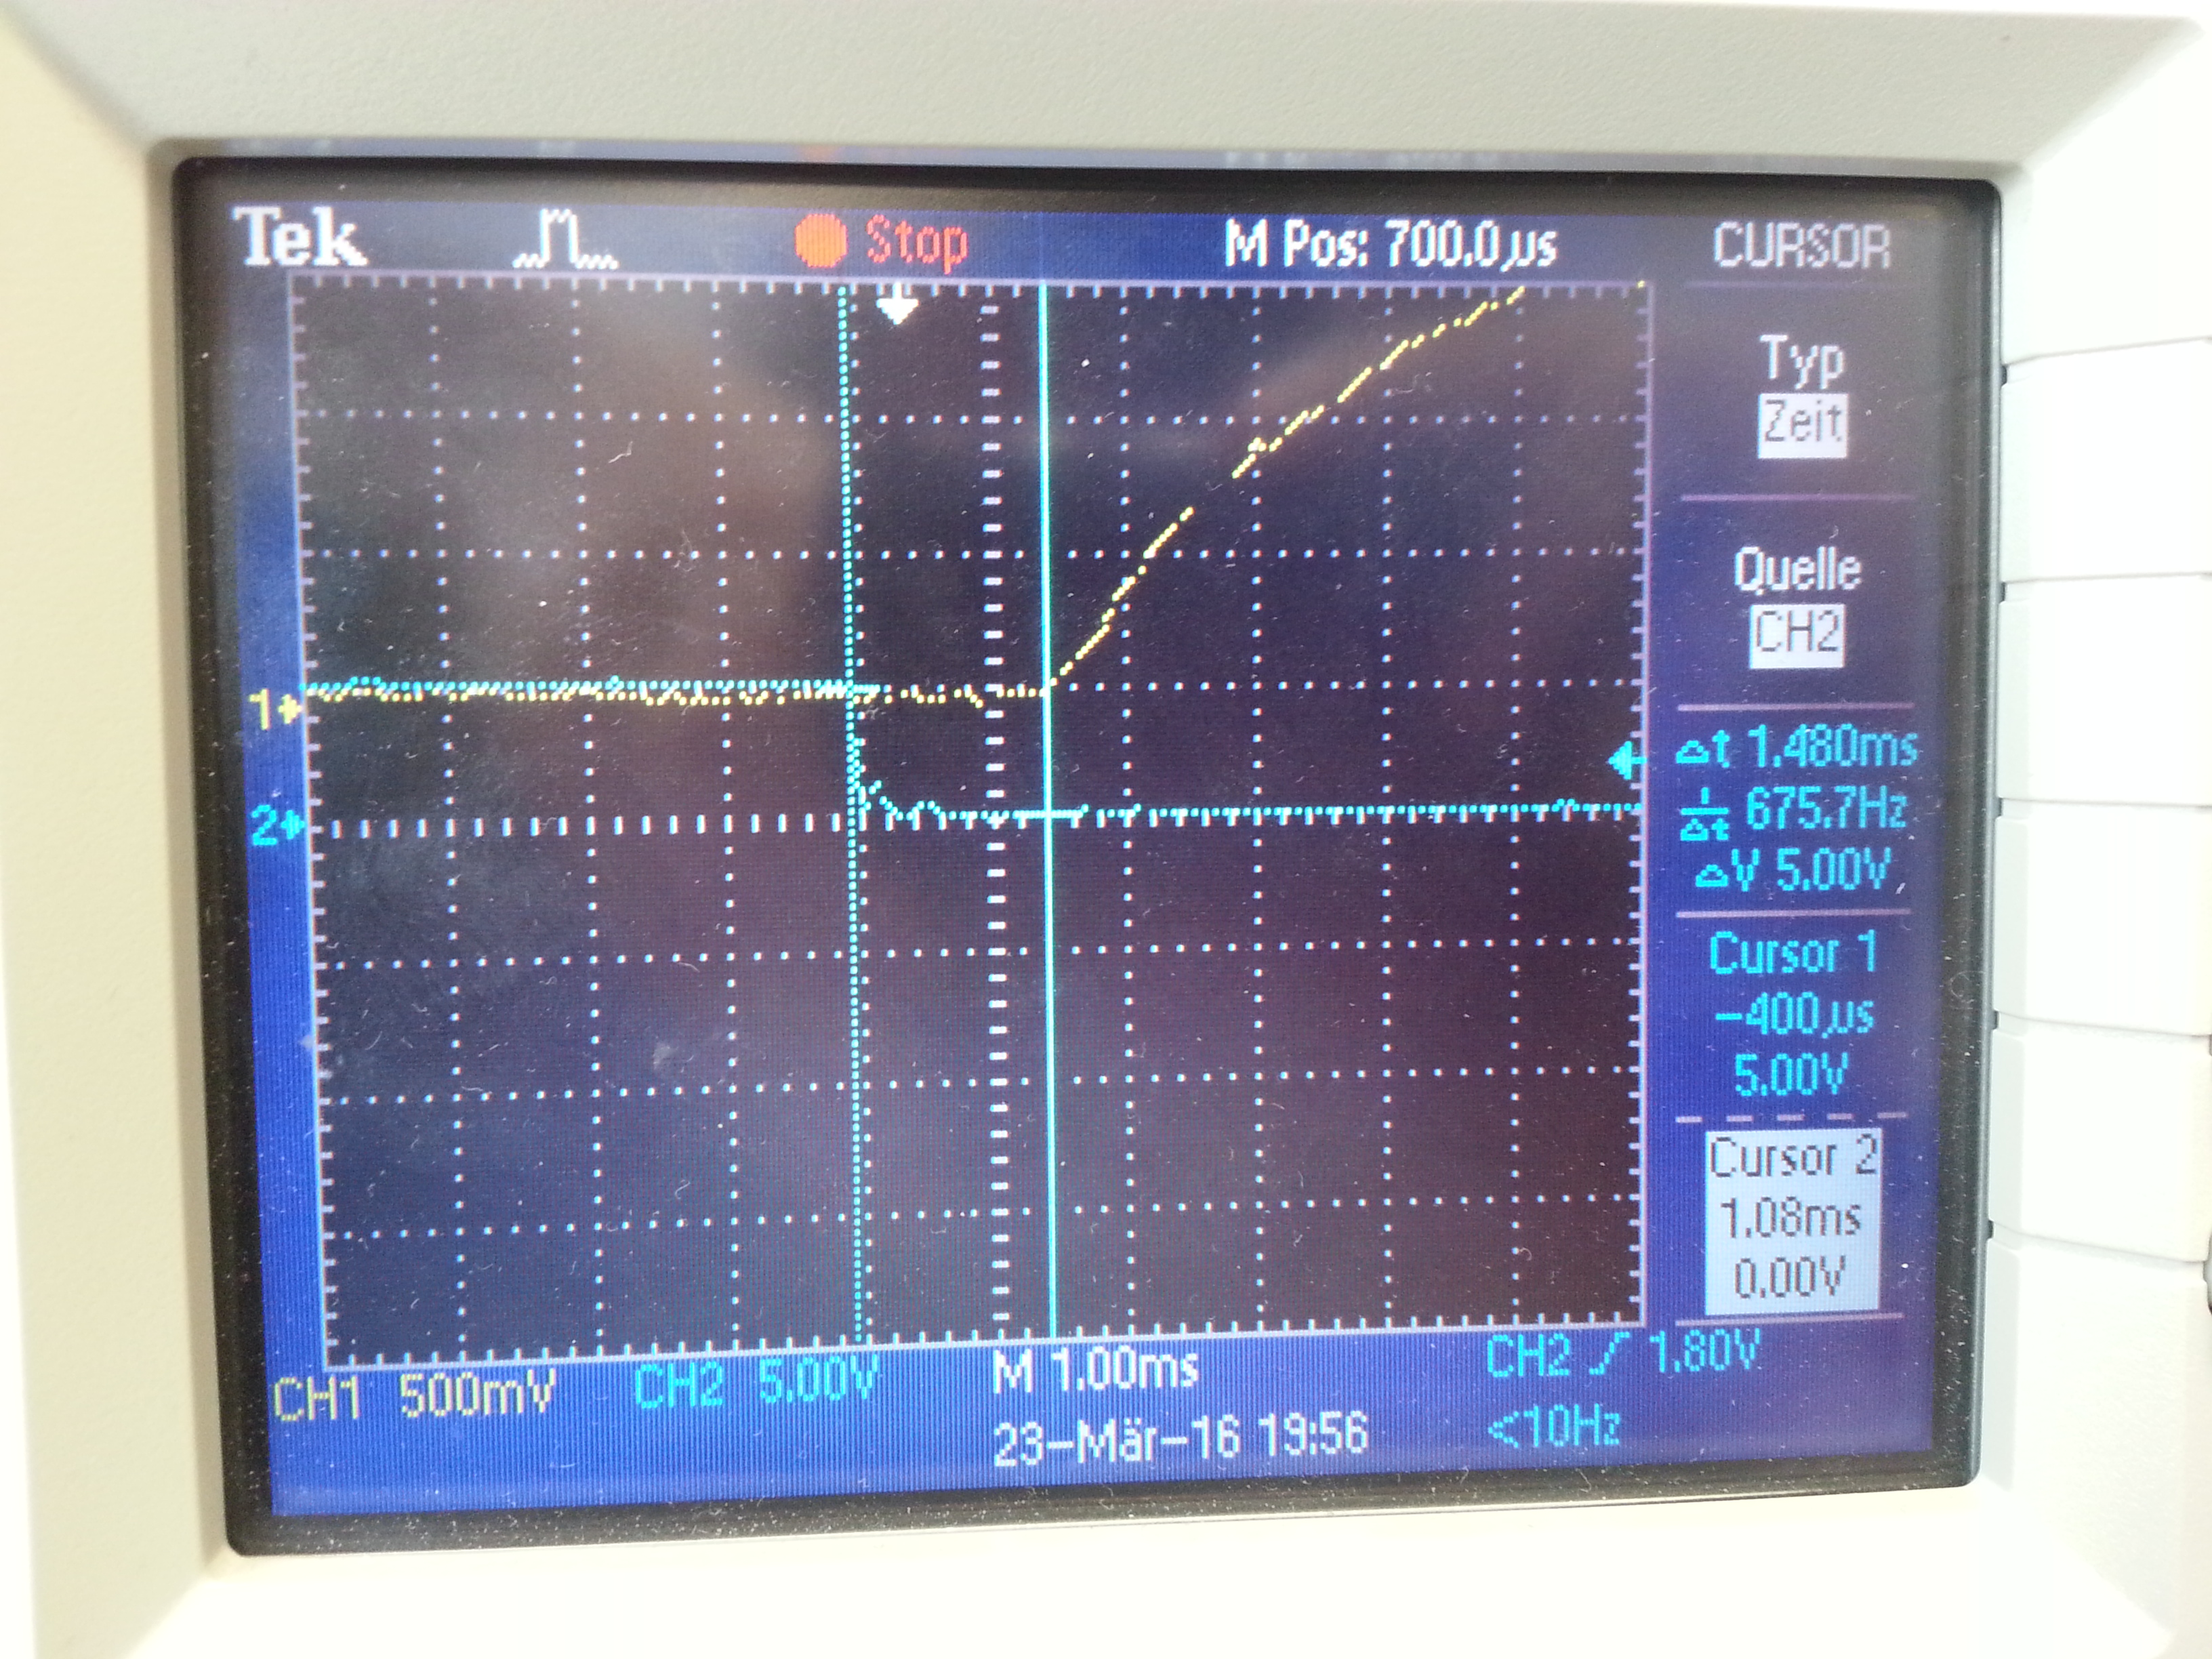
\includegraphics[scale=0.12]{Bilder/oszi.jpg}
\caption{Beispiel einer Laufzeitmessung mit dem Oszilloskop bei einem Abstand von 42.5cm}
\end{figure}
\begin{table}[H]\centering
\caption{Werte der Laufzeitmessung mit dem Oszilloskop}
\begin{tabular}{c|c}
Abstand in m & Zeitdifferenz der Spannungspeaks in ms\\ 
\hline
$42.5$& $1.48$\\ 
$34.5$& $1.24$\\
$26.5$& $1.08$\\
\end{tabular} 
\end{table}
Der Fehler auf die Zeit ergibt sich aus der Auflösung des Oszilloskops zu $0.04ms$.
Die Lufttemperatur betrug während des Versuchs ca. $22.6^{\circ}C$.
\subsubsection{Transformation der Rohdaten/Analyse}
Zur Auswertung wurden die gemessenen Werte der Cassy-Messung für die Zeit bei den jeweiligen Abständen gemittelt und die Fehler bestimmt.
\begin{table}[H]\centering
\caption{Mittelwerte der Cassy-Laufzeitmessung mit Fehlern}
\begin{tabular}{c|c|c}
Abstand in m & Mittelwert der Zeit in ms & $\sigma_t$ in ms\\ 
\hline
$42.5$& $1.51705$& $4.104 \cdot 10^{-4}$\\ 
$38.5$& $1.28692$& $7.141 \cdot 10^{-2}$\\
$34.5$& $1.08284$& $4.526 \cdot 10^{-2}$\\
$30.5$& $1.05089$& $4.390 \cdot 10^{-2}$\\
$26.5$& $0.96639$& $5.193 \cdot 10^{-4}$\\
$22.5$& $0.92490$& $3.756 \cdot 10^{-2}$\\
$18.5$& $0.80627$& $4.416 \cdot 10^{-2}$\\
\end{tabular} 
\end{table}
$~$\newline
Die Mittelwerte mit ihren Fehlern wurde anschließend gegen den Abstand des Mikrofons aufgetragen, eine Lineare Regression durchgeführt und die dazugehörigen Residuen bestimmt.
\newline
Die Auswertung der Daten des Oszilloskops erfolgte analog, nur dass wir keine Werte mitteln mussten.
\begin{figure}[H]
\centering
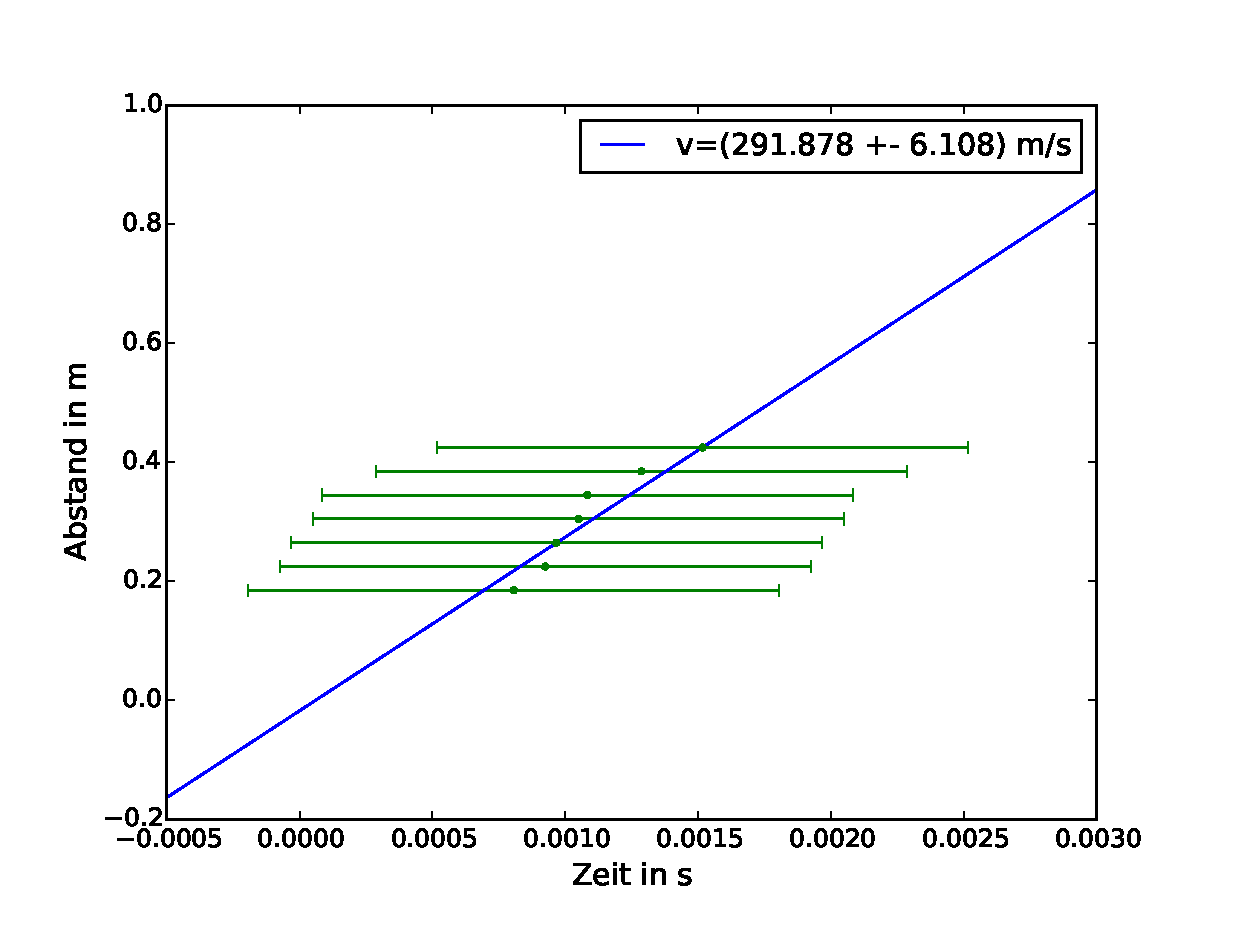
\includegraphics[scale=0.79]{Bilder/Linreg-Laufzeit.eps}
\caption{Lineare Regression durch die Mittelwerte der Cassy-Messung mit ihren Fehlern}
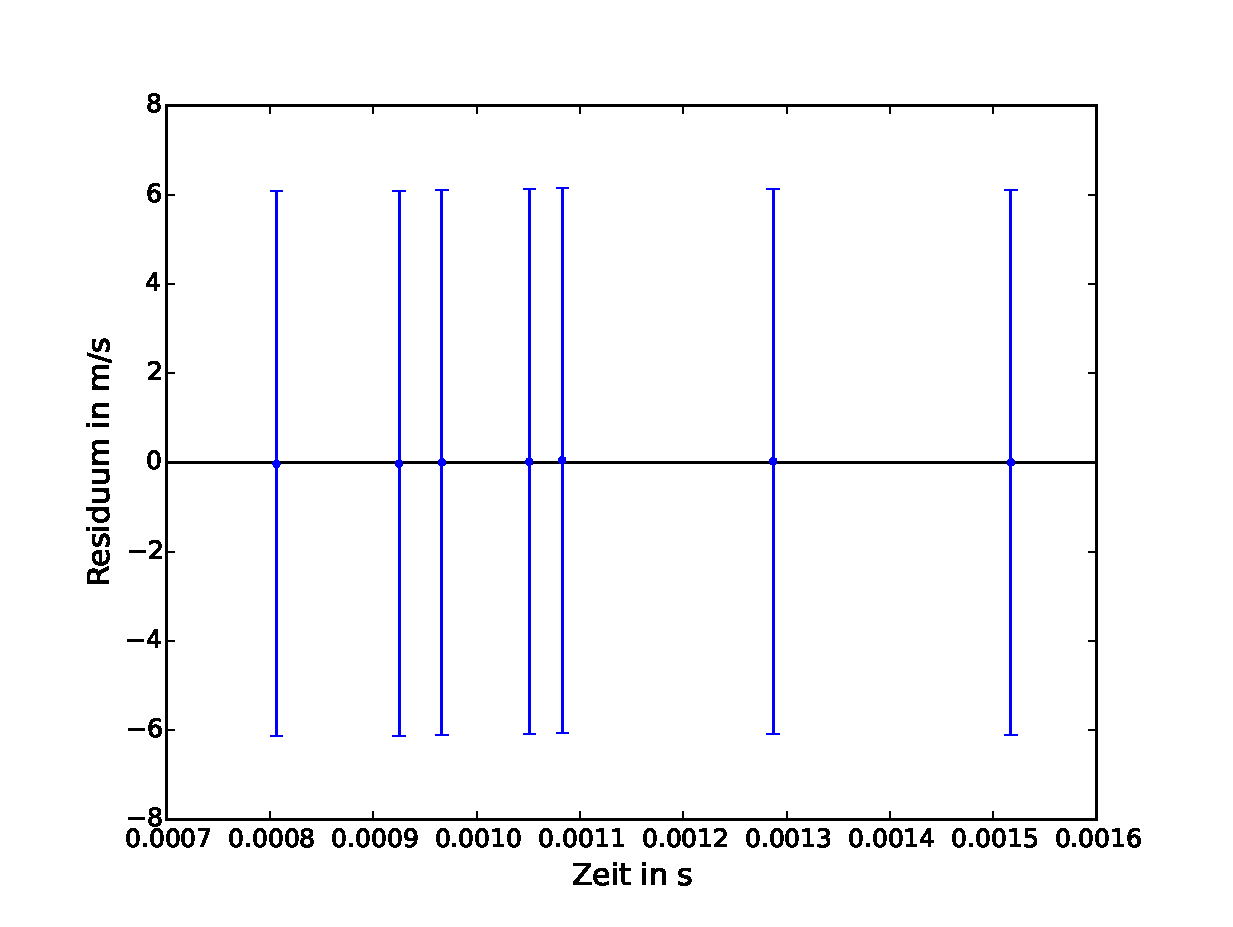
\includegraphics[scale=0.79]{Bilder/Residuen-Laufzeit.eps}
\caption{Residuen des Fits, der Cassy-Messung}
\end{figure}
\begin{figure}[H]
\centering
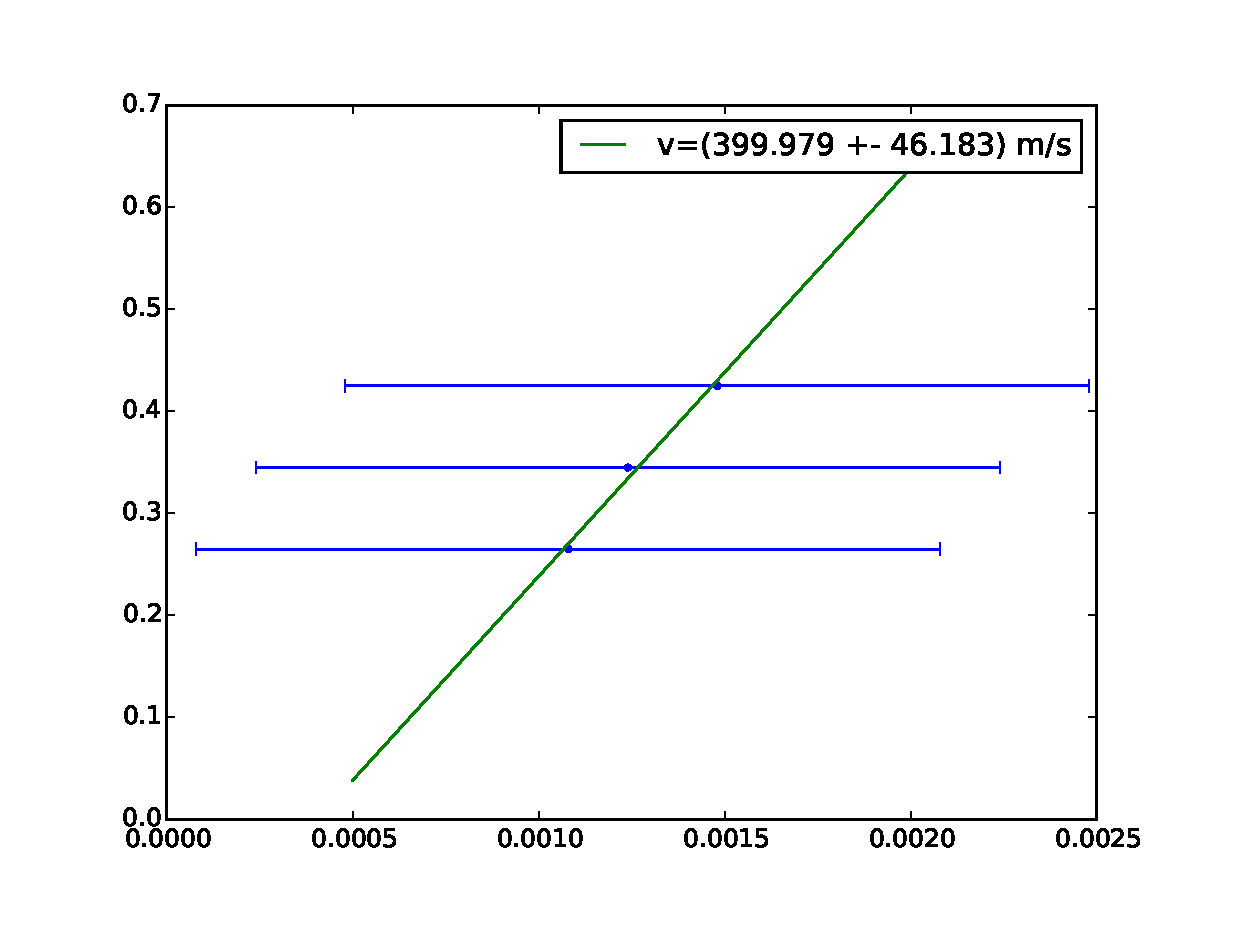
\includegraphics[scale=0.8]{Bilder/Linreg-Oszi.eps}
\caption{Lineare Regression der vom Oszilloskop abgelesenen Werte mit ihren Fehlern}
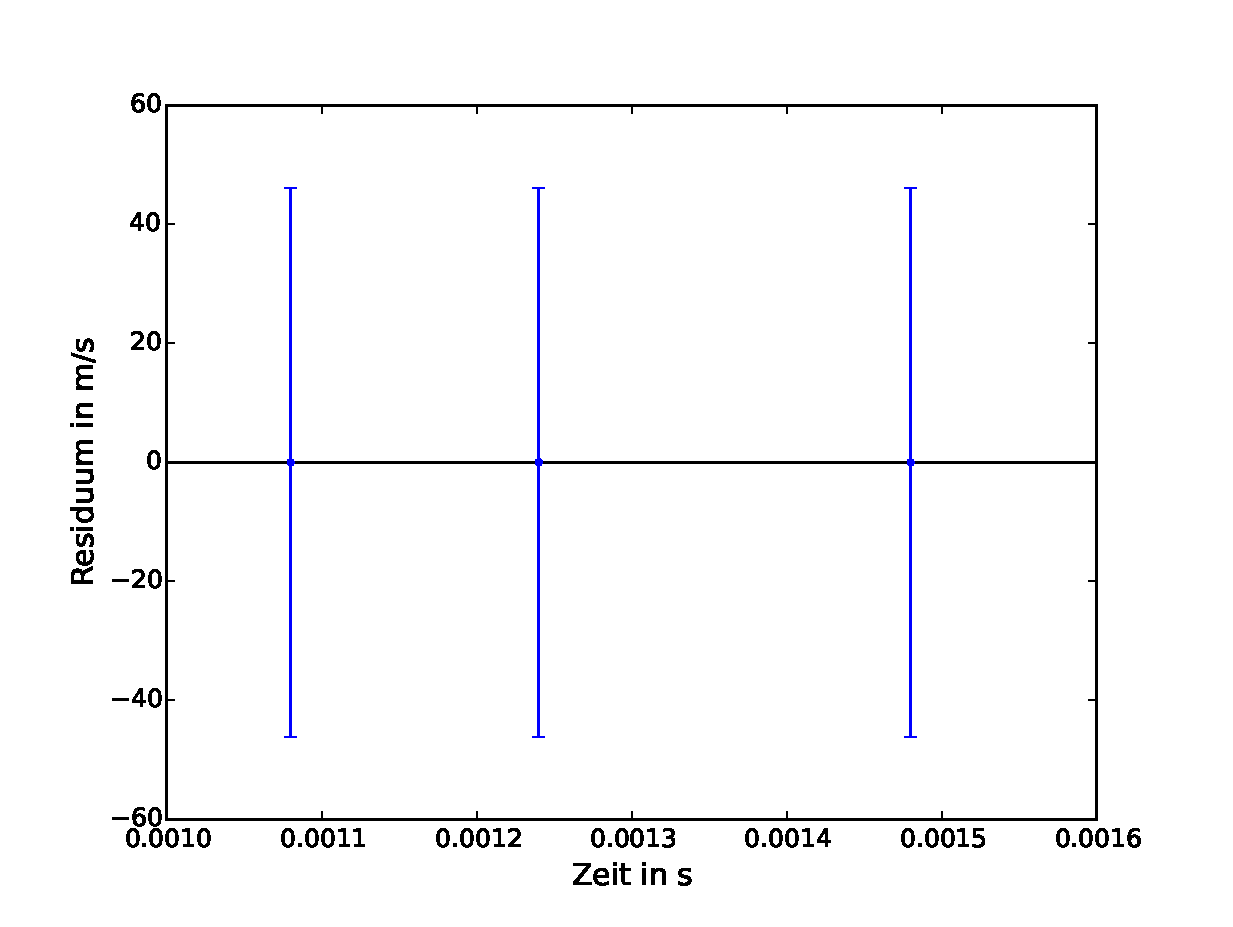
\includegraphics[scale=0.8]{Bilder/Residuen-Oszi.eps}
\caption{Residuen des Fits der Oszilloskop-Messung}
\end{figure}
$~$\newline
Als Ergebnis für die Schallgeschwindigkeit in Luft erhalten wir also einen Wert von \newline $v=(291.878 \pm 6.108) \frac{m}{s}$ für die Cassy-Messung und einen Wert von\newline $v=(399.979 \pm 46.183)\frac{m}{s}$.
\subsubsection{Fazit}
Der Literaturwert der Schallgeschwindigkeit in Luft beträgt bei einer Temperatur von $20^{\circ}C$, $342.46\, \frac{m}{s}$. Mit Gleichung (\ref{Temperaturabhängigkeit}) ergibt sich damit ein Wert von $344.98 \, \frac{m}{s}$.
Unser Ergebnis von $v=(291.878 \pm 6.108) \frac{m}{s}$ bei der Cassy-Messung weicht damit um $8\sigma$ vom Literaturwert ab. Dies erklären wir uns durch starke Streuung unserer Messwerte, bei ein und der selben Distanz (siehe Abbildung (\ref{Laufzeitrohdaten})). \newline
Unser Ergebnis von $v=(399.979 \pm 46.183)\frac{m}{s}$ bei der Oszilloskop-Messung weicht um etwas mehr als $1\sigma$ vom Literaturwert ab und ist somit völlig zufriedenstellend.
\section{Bestimmung der Schallgeschwindigkeit durch Vermessen einer stehenden Welle}
\subsection{Versuchsbeschreibung}
In diesem Versuch werden wir den Wert der Schallgeschwindigkeit über das Vermessen einer stehenden Welle bestimmen. Der Zusammenhang zwischen der Position der Bäuche der stehenden Welle, der angeregten Resonanzfrequenz und der Schallgeschwindigkeit wird durch folgende Formel beschrieben:
\begin{equation}
v_{Schall} = \lambda\cdot f
\end{equation}
Wir werden den Schalldruck an verschiedenen Stellen innerhalb des Rohres bei einer stehenden Welle messen. Danach tragen wie die Amplitude des Schalldrucks gegen die Strecke auf und suchen die Extrema. Diese Punkte werden dann in einer Linearen Regression verwendet. Die Steigung gibt uns $\frac{\lambda}{2}$ zurück, daraus können wir dann zusammen mit der bereits eingestellten Frequenz die Schallgeschwindigkeit berechnen.

\subsection{Versuchsaufbau und Durchführung}
Verwendete Geräte:
\begin{itemize}
\item Frequenzgenerator
\item Sensor-Cassy
\item Richtmikrofon
\item Lautsprecher
\item Rohr ($0.425\, m \pm 0.001\,$m (Messfehler auf Massband))
\item Massband ($\sigma_{Massband} = 0.001\, m$)
\end{itemize}
Wir haben unser Cassy mit folgenden Einstellungen verwendet:
\begin{itemize}
\item Kanal A / Spannung UA1 / $-10..10\, V$ /
\item Kanal B / Timerbox / Frequenz fb1(E) / $5000\, Hz$ / Torzeit: $1\, s$
\item manuelle Messung
\item Darstellung: X-Achse n / Y-Achse Ua1
\end{itemize}
Den Frequenzgenerator haben wir wie folgt eingestellt:
\begin{itemize}
\item Signalform / $\sim$ (Sinusschwingung)
\item Bereich / $x1k (0.2 - 2.4 x 1\, $kHz$)$
\item $\sigma_f = 10\,$Hz (Abschätzung durch ungenaue Feinabstimmung, gerätbedingt)
\item Offset / 0
\item Amplitude / mittig
\end{itemize}
Die Raumtemperatur betrug $23^{\circ}\, C$.
\begin{figure}[H]
\centering
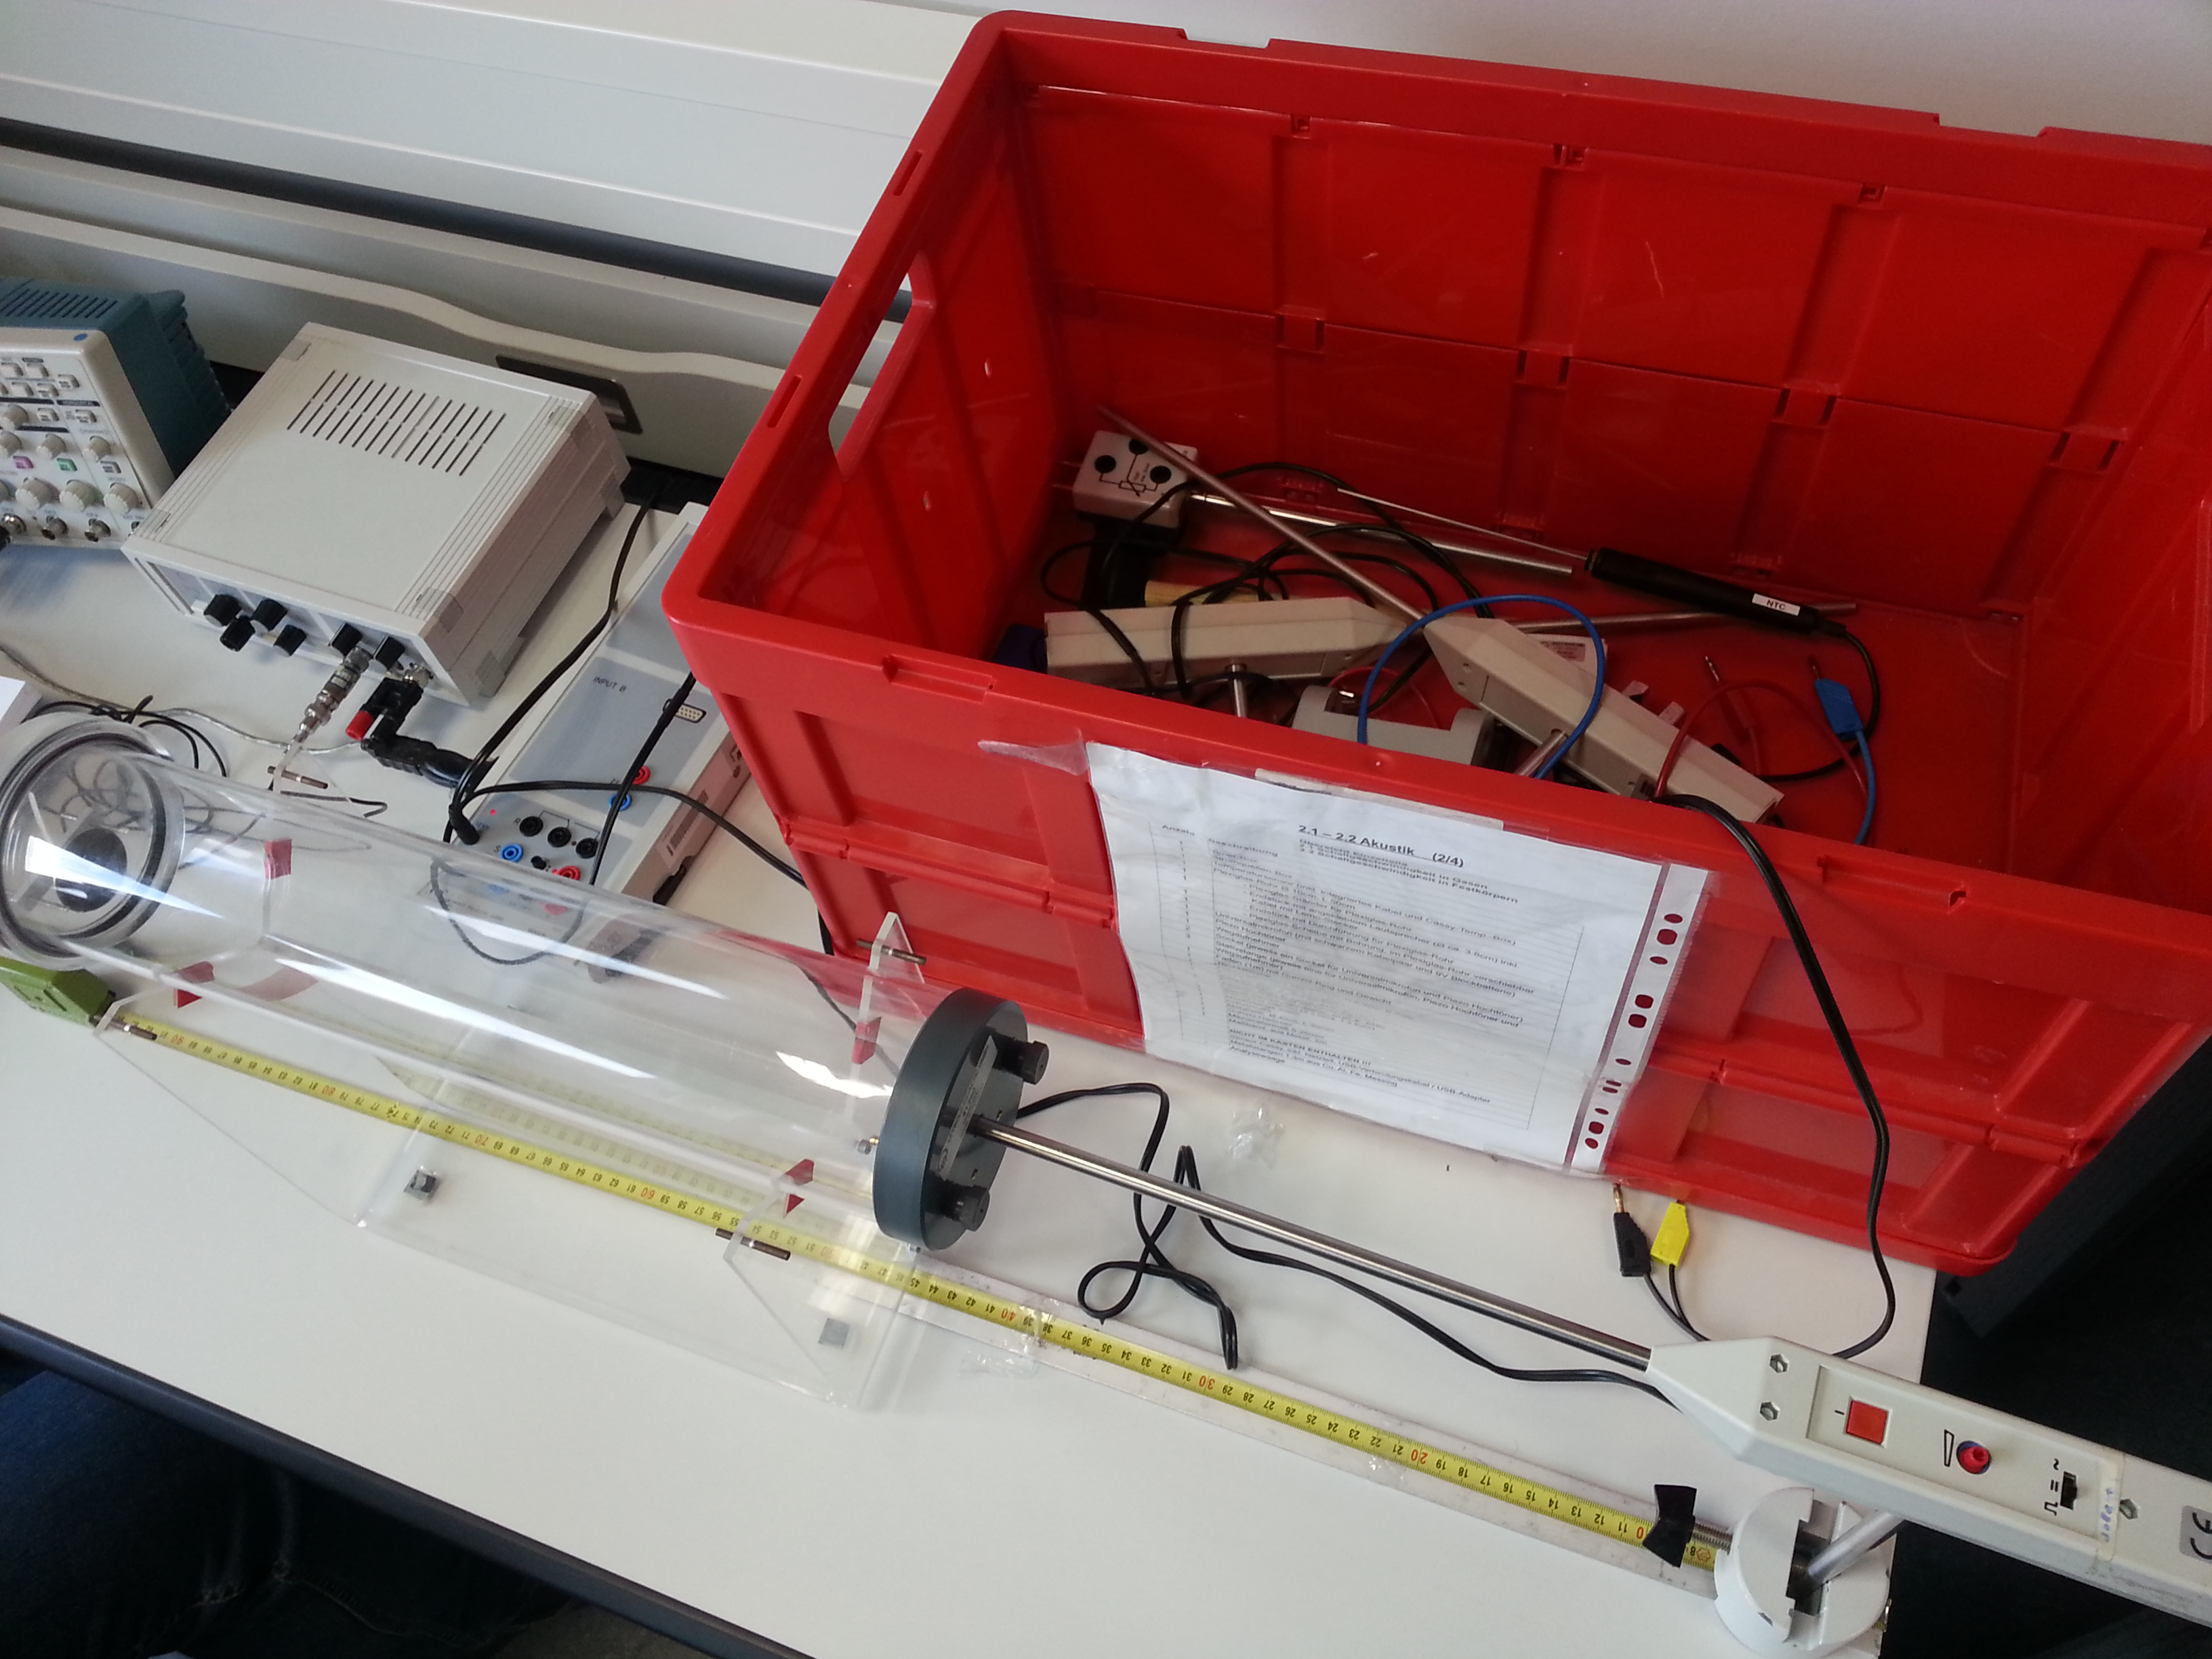
\includegraphics[scale=0.1]{Bilder/Druckknoten-Messung3.jpg}
\caption{Versuchsaufbau für die Bestimmung der Schallgeschwindigkeit über die Vermessung einer stehenden Welle}
\end{figure}
Durchführung:\newline
Wir messen alle 0.5$\,$cm angefangen bei 2.5$\,$cm (gemessen vom Anfang der Schiene). Die Umrechnung von n in m lautet also wie folgt:
\begin{equation}
l = (0.025 + n\cdot 0.005) - 0.425
\end{equation}
wobei die 42.5$\,$cm die Länge des Rohres beschreibt, wie unter Geräte angegeben.
Die sich so ergebenen Daten sehen wie folgt aus:
\begin{figure}[H]
\centering
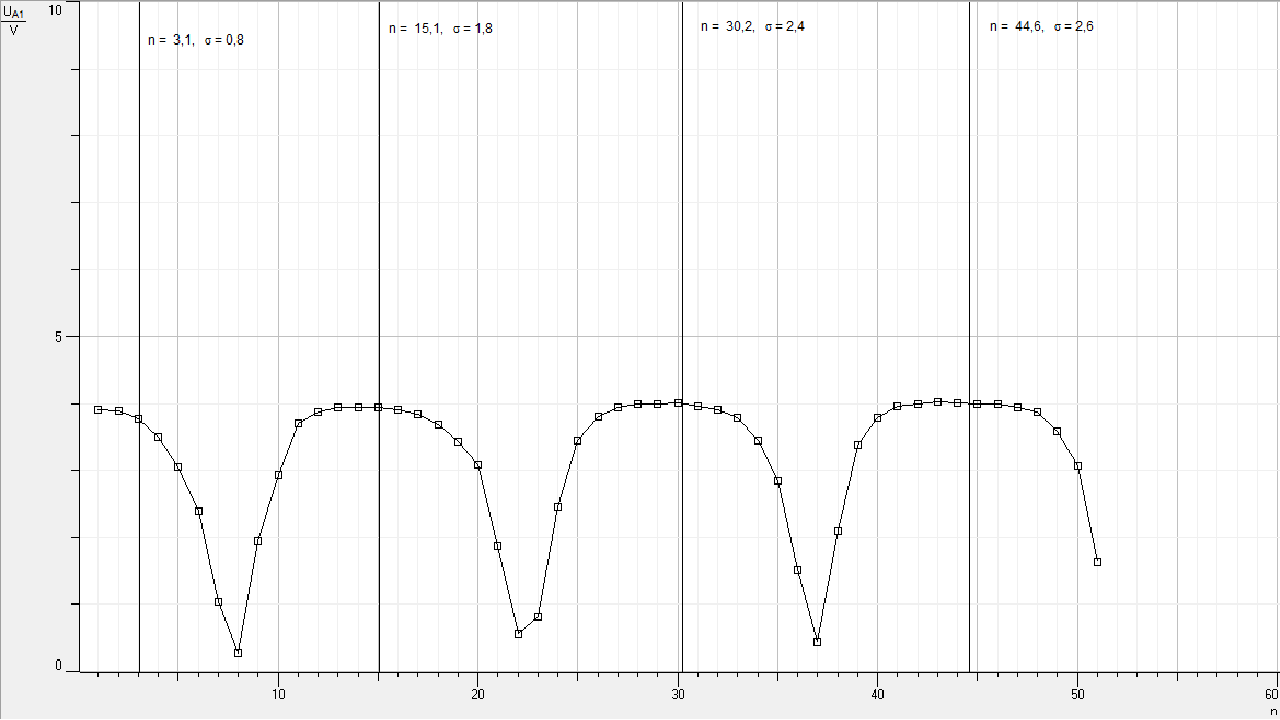
\includegraphics[scale=0.3]{Bilder/baeuche.png}
\caption{Amplitude des Schalldrucks aufgetragen gegen eingeführte Länge des Richtmikrofons (in n - Umrechnung siehe oben)}
\end{figure}
Wir haben leider wenig Punkte bei den Knoten, daher werden wir für unsere Lineare Regression nur unsere Peaks betrachten. Diese bestimmen wir mit der Peaksschwerpunktfunktion von Cassy.
Die sich daraus ergebenen Daten sind unter Rohdaten aufgeführt.

\subsection{Versuchsauswertung}

\subsubsection{Rohdaten}
\begin{table}[H]
\begin{tabular}{c|c|c}
Position Bauch N & Messpunkt n & Länge [m] \\ 
\hline 
1.5 & 1 & 0.395 \\ 
2.5 & 15 & 0.325 \\ 
3.5 & 30 & 0.25 \\ 
4.5 & 45 & 0.175 \\ 
\end{tabular}
\caption{Druckbäuche für $f = 2400\,$Hz, mit $\sigma_l = 0.0028\,$m}
\end{table}
\subsubsection{Transformation der Rohdaten}
Mit den oben genannten Rohdaten führen wir jetzt eine Lineare Regression durch. Die Steigung der Linearen Regression gibt uns $\frac{\lambda}{2}$ zurück und beträgt $0.0735\,$m. Unsere Lineare Regression sieht wie folgt aus:
\begin{figure}[H]
\centering
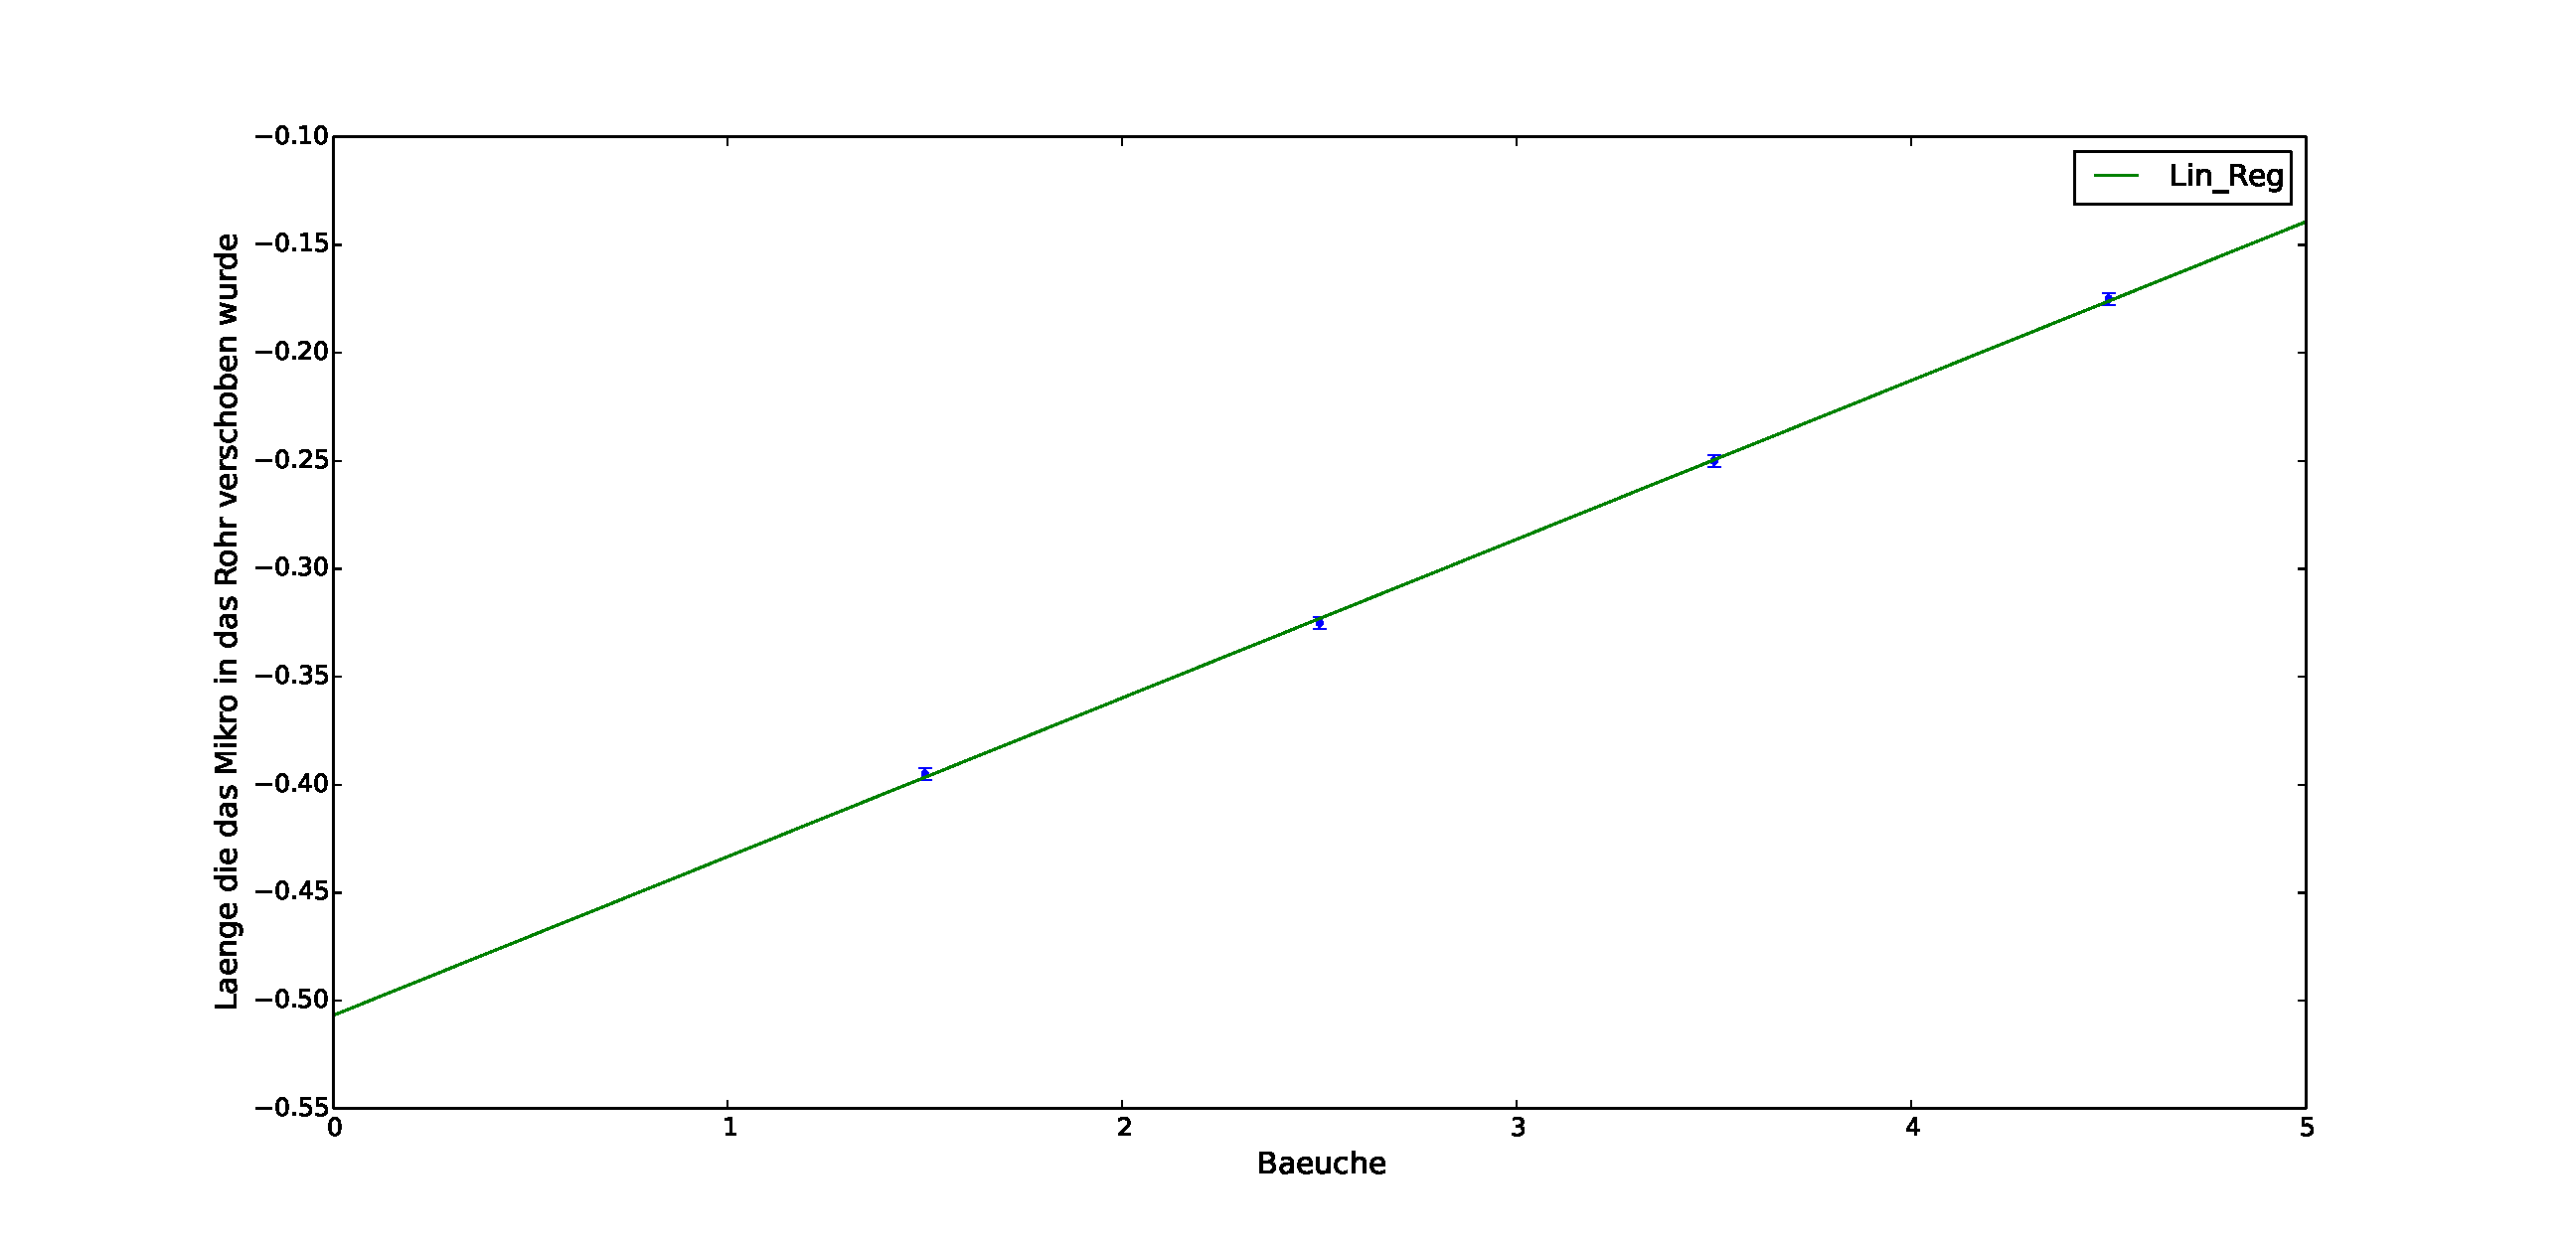
\includegraphics[scale=0.3]{Bilder/linreg_stehende_welle.eps}
\caption{Lineare Regression der 4 oben genannten Peaks, die Steigung beträgt $\frac{\lambda}{2}$}
\end{figure}
Wir haben dabei ein $\chi^2 = 0.47$ erreicht.
Unser Residuenplot dazu sieht wie folgt aus:
\begin{figure}[H]
\centering
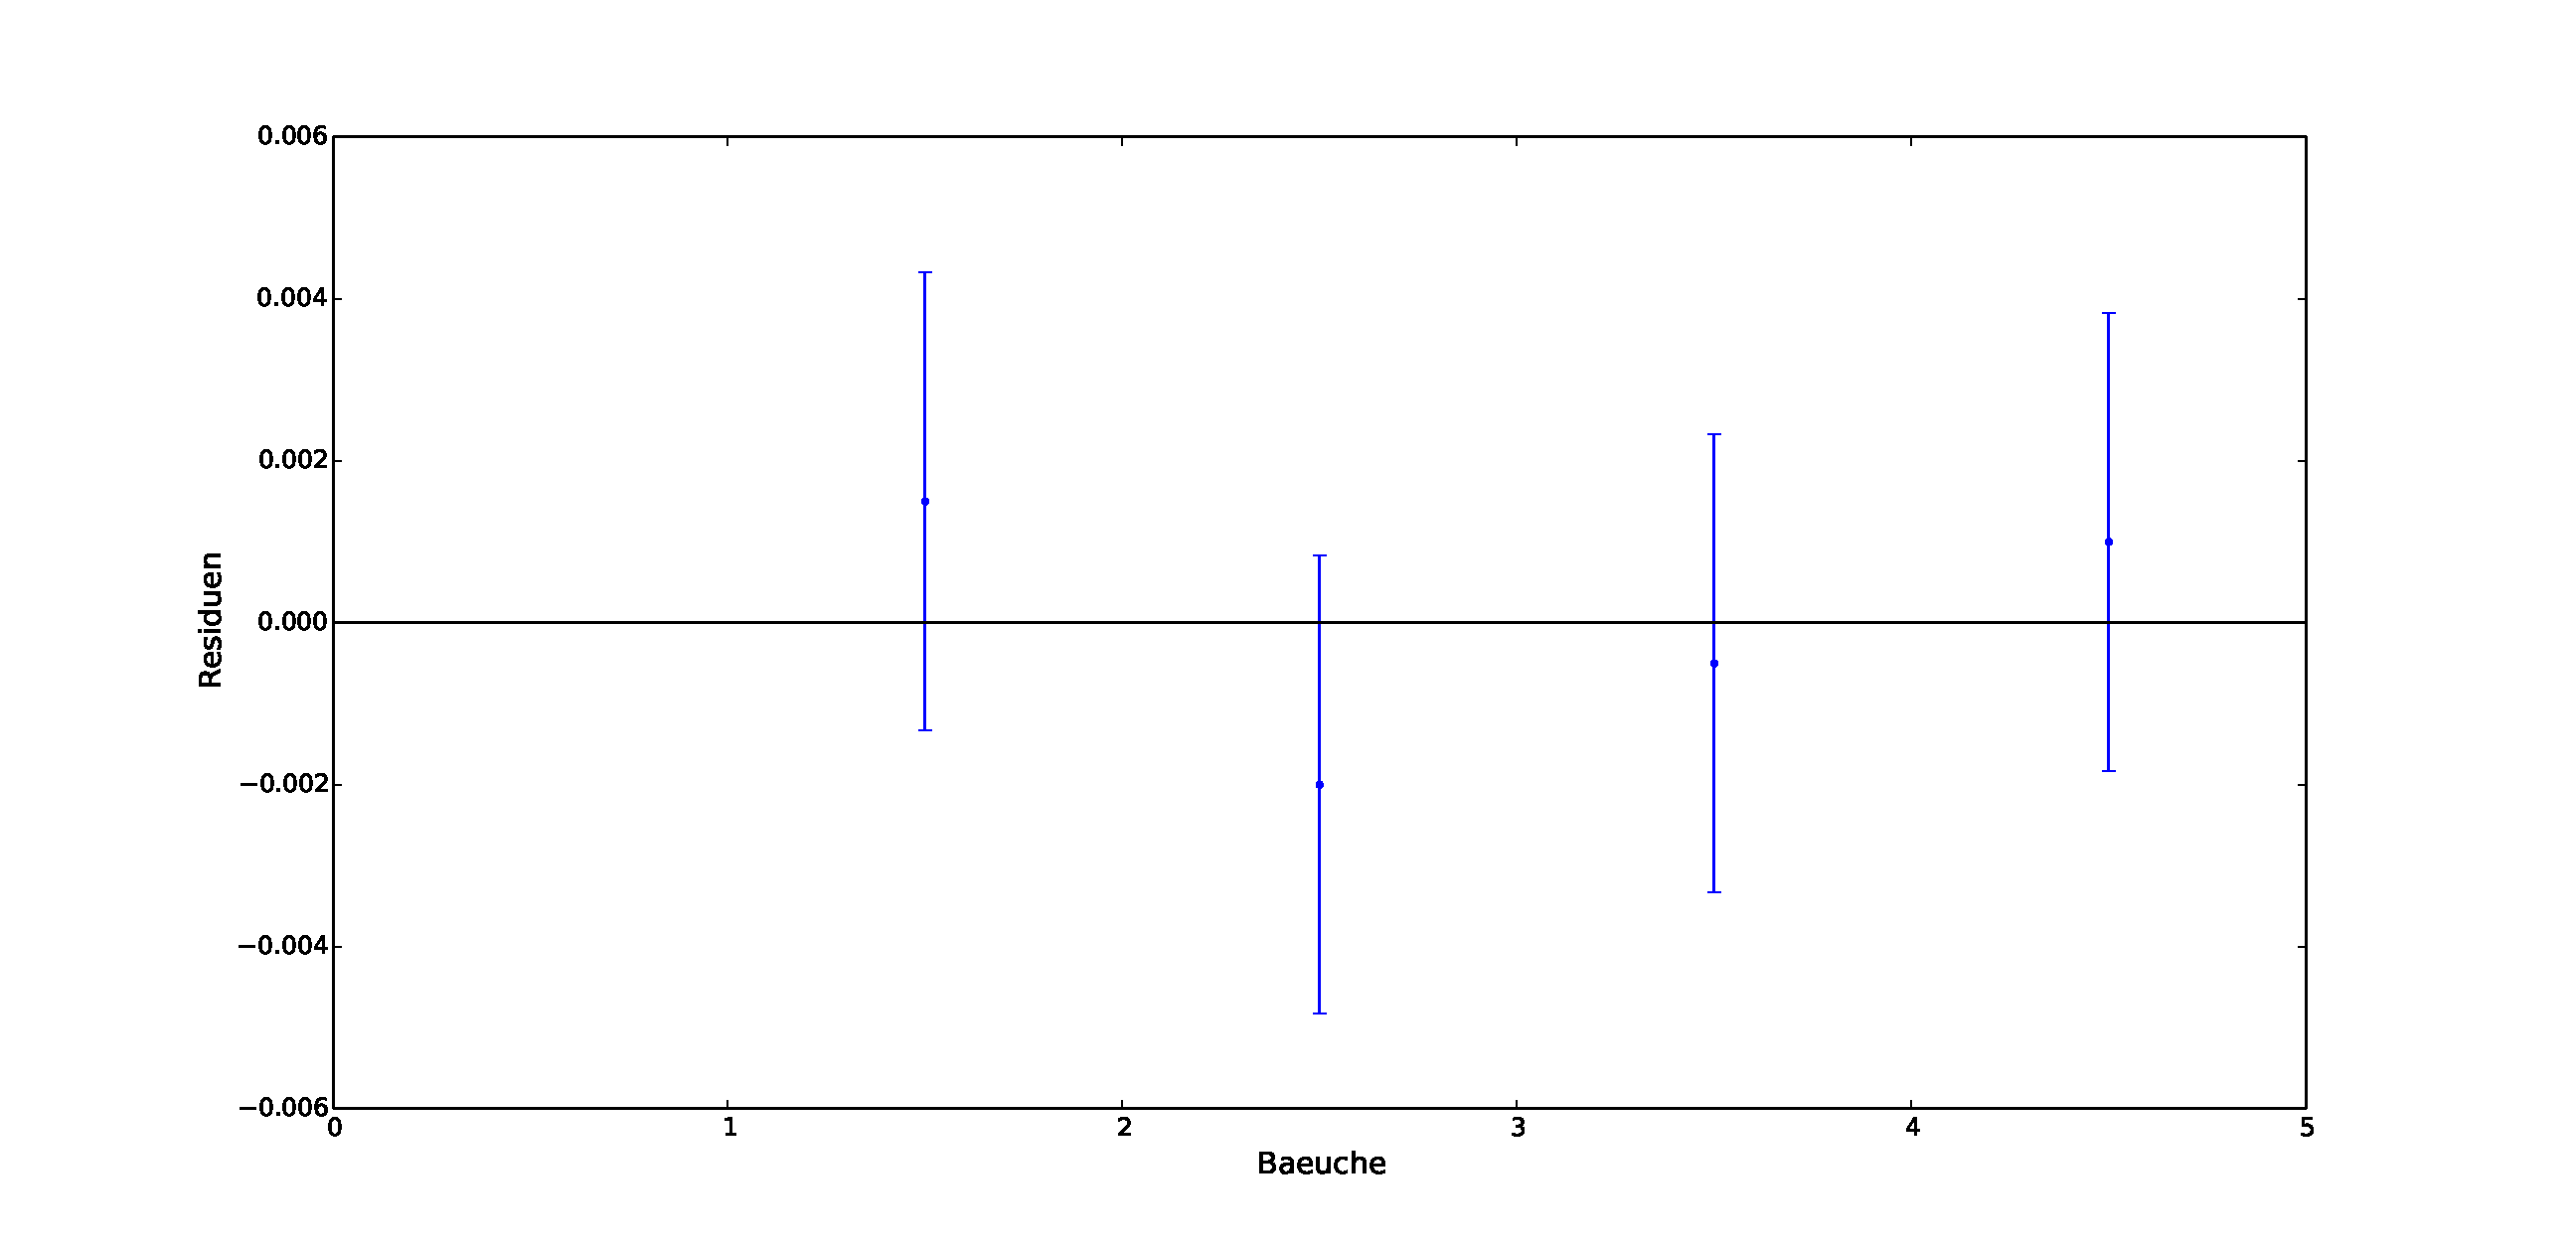
\includegraphics[scale=0.3]{Bilder/residuen_stehende_welle.eps}
\caption{Residuenplot (Daten - Fit) mit den jeweiligen Fehlern}
\end{figure}
Alle Werte liegen mit ihren Fehlern in einem Abstand kleiner als $\sigma$ von 0 entfernt. Die Werte sind gleichverteilt um 0 gestreut und es lässt sich keine Systematik erkennen.\newline
Um auf unseren Wert für $v$ zu kommen müssen wir die eingestellte Frequenz $f = 2400\,$Hz und die mit dem Faktor 2 multiplizierte Steigung (wir erinnern uns, dass die Steigung der Linearen Regression nur $\frac{\lambda}{2}$ zurückgab) der Linearen Regression in die am Anfang dieses Kapitels eingeführte Gleichung
\begin{equation*}
v = \lambda\cdot f
\end{equation*}
einsetzen. So erhalten wir einen Wert für $v = 352.8\,\frac{m}{s}$.
Um den Fehler auf $v$ zu erhalten, müssen wir $\sigma_{\lambda}$ und $\sigma_f$ fortpflanzen.
\begin{equation}
\sigma_{v} = \sqrt{f^2\cdot\sigma_{\lambda}^2 + \lambda^2\cdot\sigma_{f}^2}
\end{equation}
mit $\sigma_{\lambda} = 0.0025\,$m (aus Ausgabe der Linearen Regression.)
Daraus ergibt sich für unser Ergebnis, dass die Schallgeschwindigkeit $v_{Schall} = 352.8 \pm 4.5\,\frac{m}{s}$ beträgt.

\subsection{Fazit}
Unser Ergebnis für die Schallgeschwindigkeit liegt innerhalb von 2$\sigma_{v}$ über dem Literaturwert (bei T$ = 20^{\circ}\,$C beträgt die Schallgeschwindigkeit $v = 343.\,\frac{m}{s}$, umgerechnet für T$ = 22.6^{\circ}\,$C mit $v = v_0\cdot\sqrt{\frac{T}{T_0}}$, $v = 344.98\,\frac{m}{s}$). Wir erklären uns diese Abweichung durch die fehlenden Werte für die Druckknoten der stehenden Welle in der Linearen Regression. Ansonsten sind wir sowohl mit unserer Anpassung ($\chi^2 = 0.47$) als auch mit der um 0 gleichverteilt gestreuten Residuen zufrieden.
\section{Vermessung der Schallgeschwindigkeit durch Variation der Frequenz}
\subsection{Versuchsberschreibung}
In diesem Versuch werden wir die Schallgeschwindigkeit aus der Steigung der Geraden 
\begin{equation}
f_n = \frac{n\cdot v}{2\cdot L}
\end{equation}
bestimmen. Dabei steht $f_n$ für die Resonanzfrequenzen, n für die Vielfache, v für die Schallgeschwindigkeit und L für die Länge des Rohres. Dafür vermessen wir zunächst grob die Resonanzfrequenzen.
Danach werden wir das gleiche noch einmal genau wiederholen, aber mit deutlich mehr Messpunkten um die jeweiligen Resonanzfrequenzen (siehe Bild), insgesamt 3 mal.

\subsection{Versuchsaufbau und Durchführung}
Verwendete Geräte:
\begin{itemize}
\item Frequenzgenerator
\item Sensor-Cassy
\item Richtmikrofon
\item Lautsprecher
\item Rohr ($0.425\, m \pm 0.001\,$ m (Messfehler auf Massband))
\item Massband ($\sigma_{Massband} = 0.001\, m$)
\end{itemize}
Wir haben unser Cassy mit folgenden Einstellungen verwendet:
\begin{itemize}
\item Kanal A / Spannung UA1 / $-10..10\, V$ /
\item Kanal B / Timerbox / Frequenz fb1(E) / $5000\, Hz$ / Torzeit: $1\, s$
\item manuelle Messung
\item Darstellung: X-Achse fb1 / Y-Achse Ua1
\end{itemize}
Den Frequenzgenerator haben wir wie folgt eingestellt:
\begin{itemize}
\item Signalform / $\sim$ (Sinusschwingung)
\item Bereich / $x1k (0.2 - 2.4 x 1\, $kHz$)$
\item $\sigma_f = 10\,$Hz (Abschätzung durch ungenaue Feinabstimmung, gerätbedingt)
\item Offset / 0
\item Amplitude / mittig
\end{itemize}
\begin{figure}[H]
\centering
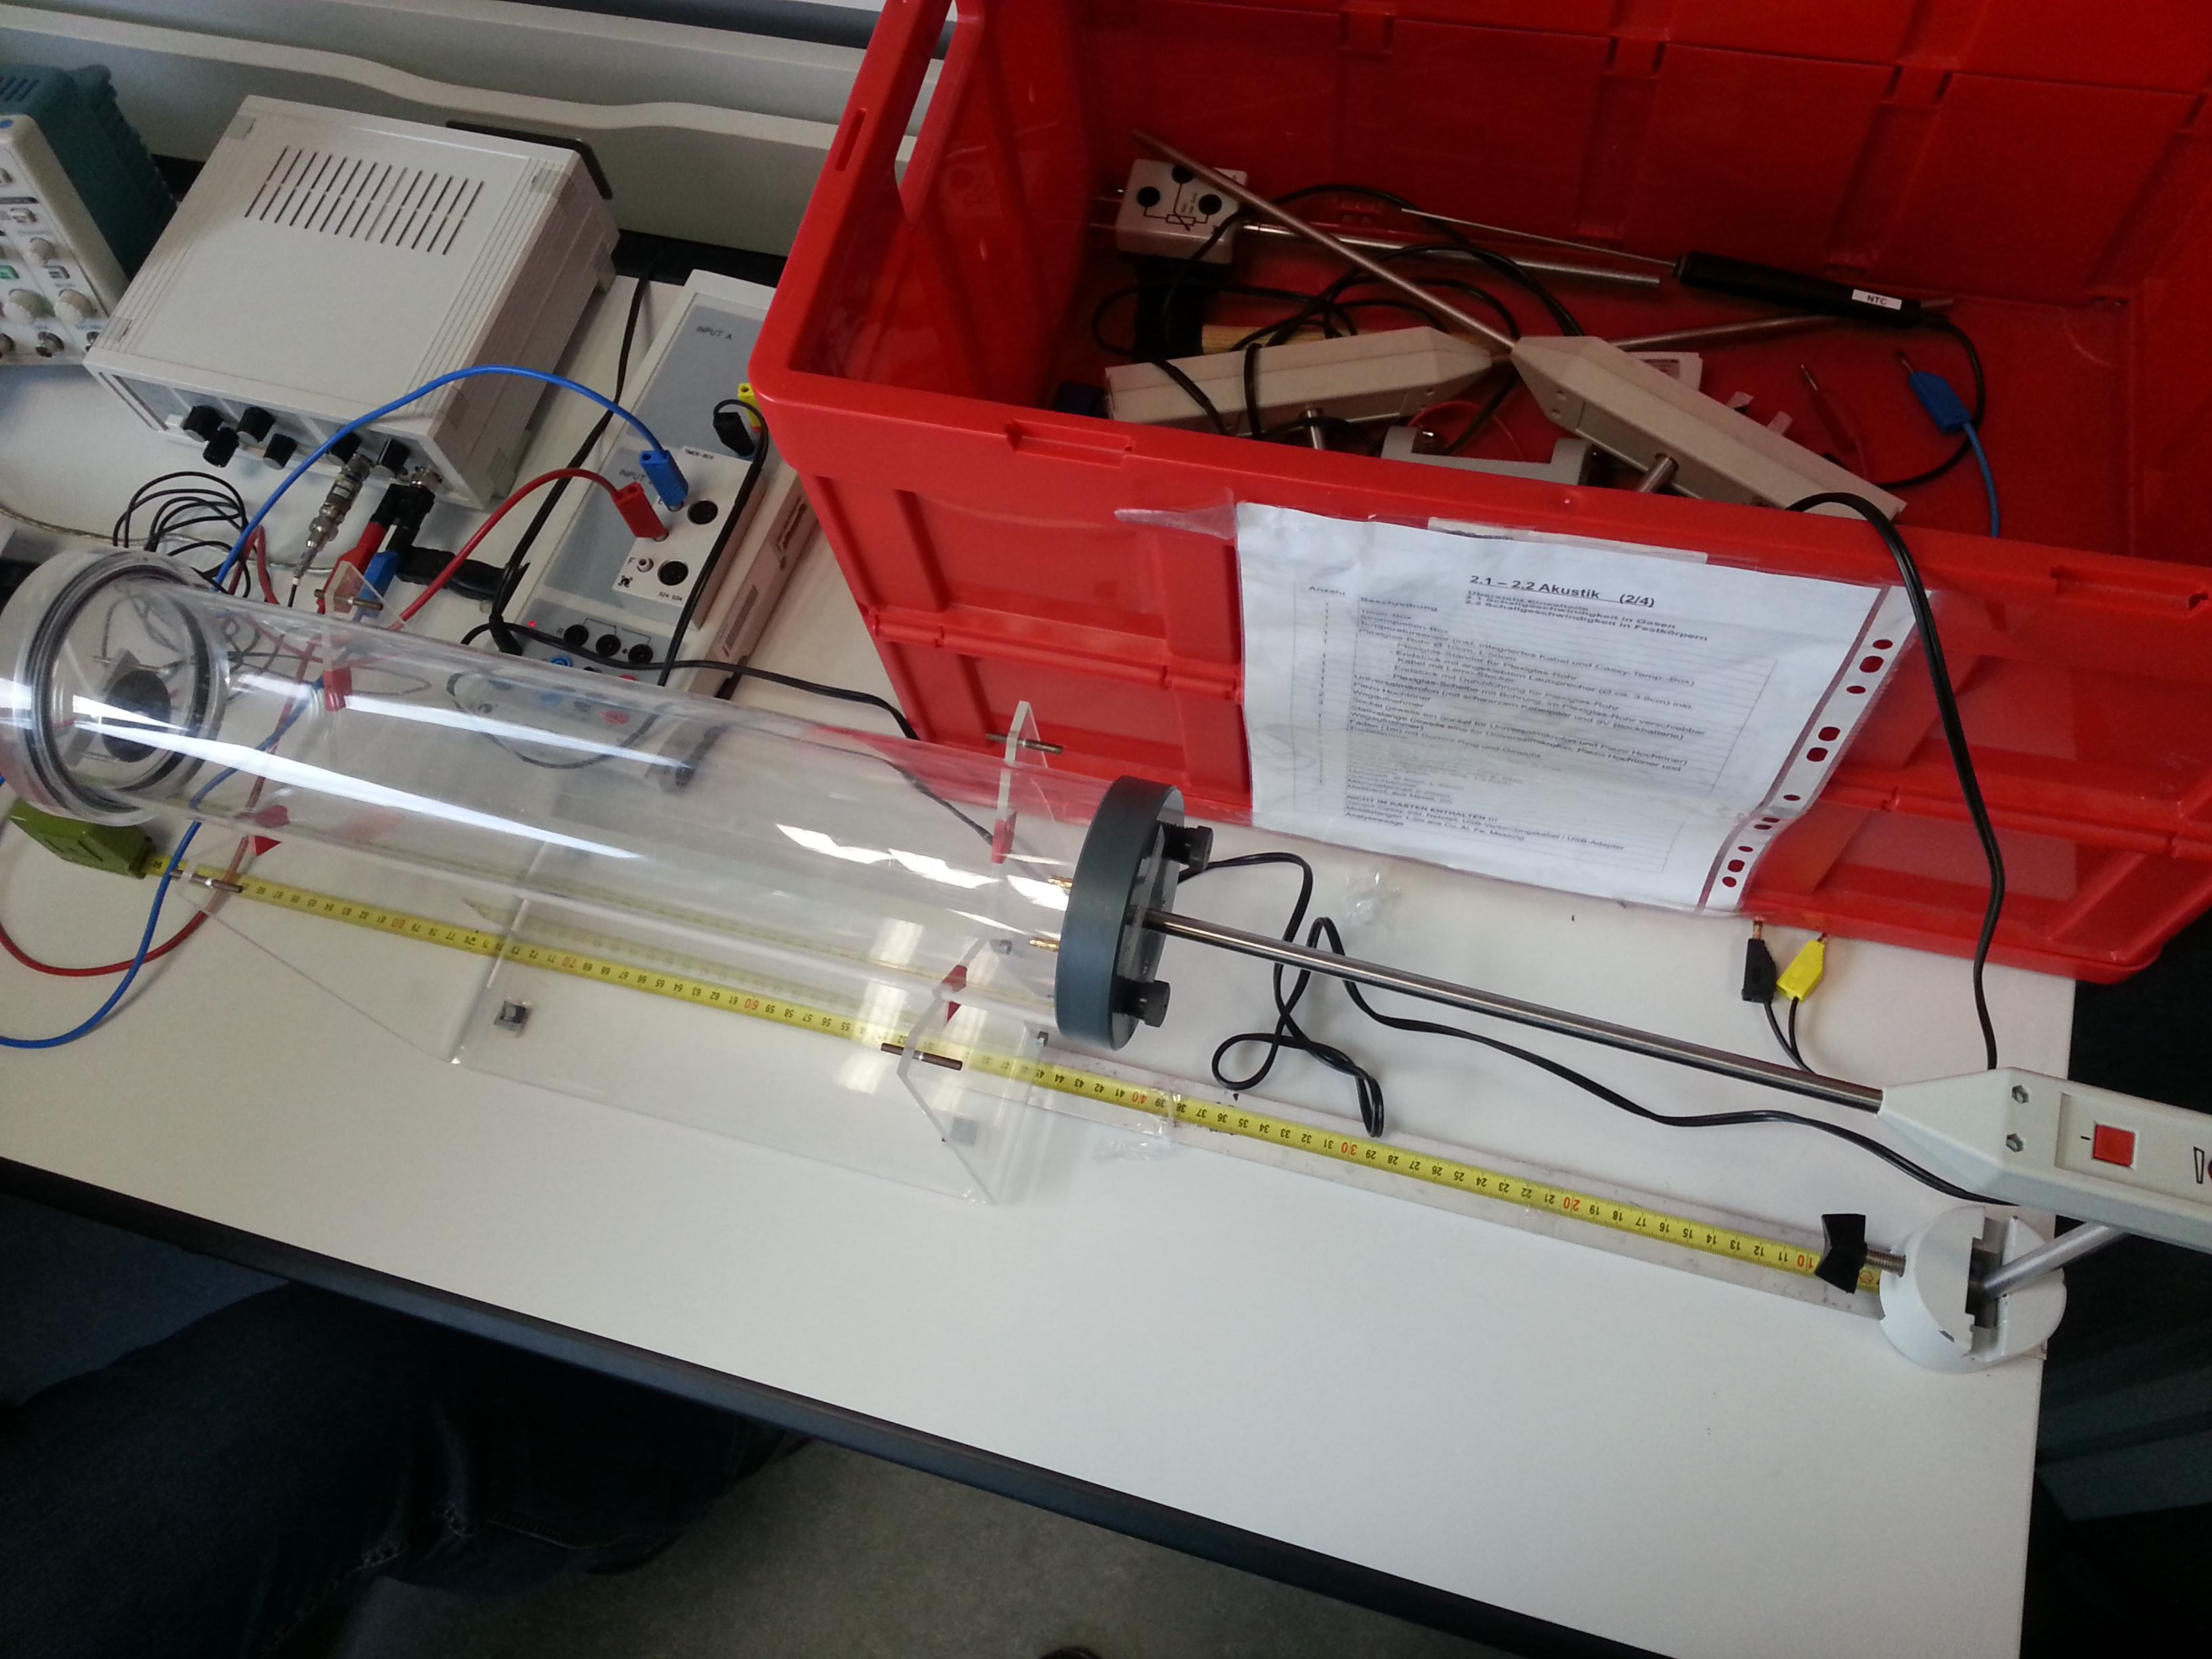
\includegraphics[scale=0.15]{Bilder/Frequenzvariation3.jpg}
\caption{Versuchsaufbau zur Messung der Schallgeschwindigkeit durch Variation der Resonanzfrequenzen}
\end{figure}
Zunächst haben wir grob die Resonanzfrequenz bestimmt:
\begin{figure}[H]
\centering
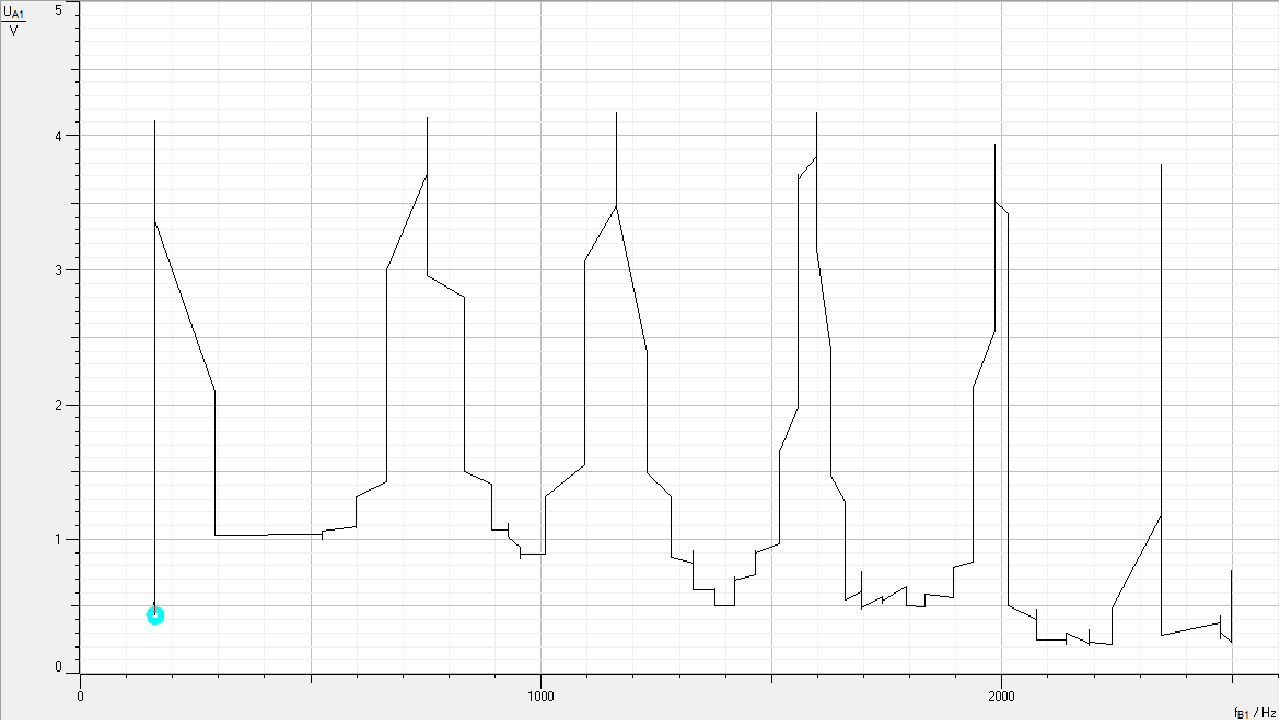
\includegraphics[scale=0.5]{Bilder/grobevermessung.png}
\caption{Grobe Vermessung der Resonanzfrequenzen - die deutlich ausgeprägten Peaks werden später genauer untersucht.}
\end{figure}
Danach haben wir an den oben zu sehenden Peaks das ganze noch mal mit mehr Messpunkten in drei Messungen gemessen:
\begin{figure}[H]
\centering
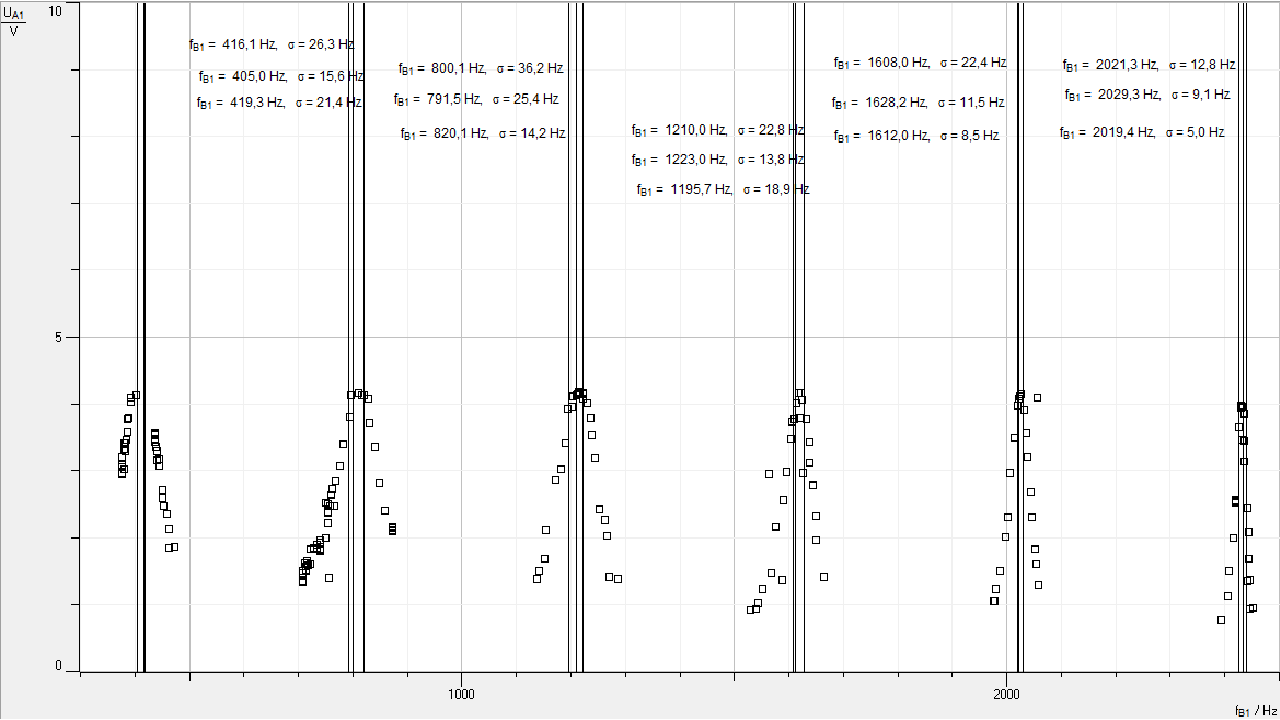
\includegraphics[scale=0.5]{Bilder/vermessung_variation_genau.png}
\caption{genaue Vermessung der Peaks an einer Beispiel Messung}
\end{figure}
Die sich daraus ergebenen Daten sind unter Rohdaten aufgeführt.
\subsection{Versuchsauswertung}
\subsubsection{Rohdaten}
\begin{table}[H]
\begin{tabular}{c|c|c|c|c|c|c}
vermutete Resonanzfrequenz & 400 & 800 & 1200 & 1600 & 2000 & 2400 \\ 
\hline 
Peak Messung I & 416.0 & 822.5 & 1210.0 & 1608.0 & 2031.1 & 2433.4 \\  
$asym_r$ Peak Messung I & 417.0 & 826.8 & 1212.6 & 1629.6 & 2041.4 & 2443.7 \\  
$asym_l$ Peak Messung I & 404.9 & 798.2 & 1190.0 & 1573.9 & 2019.3 & 2425.5 \\ 
\hline 
Peak Messung II & 420.7 & 822.1 & 1210.9 & 1620.0 & 2037.2 & 2446.7 \\  
$asym_r$ Peak Messung II & 423.0 & 836.4 & 1216.5 & 1631.3 & 2047.8 & 2467.3 \\ 
$asym_l$ Peak Messung II & 404.3 & 797.5 & 1194.0 & 1612.3 & 2013.8 & 2421.3 \\ 
\hline 
Peak Messung III & 416.1 & 800.1 & 1210.0 & 1612.0 & 2019.4 & 2433.4 \\  
$asym_r$ Peak Messung III & 419.3 & 820.1 & 1223.0 & 1628.2 & 2029.3 & 2439.2 \\  
$asym_l$ Peak Messung III & 405.0 & 791.5 & 1195.7 & 1608.0 & 2019.4 & 2425.5
\end{tabular}
\caption{Vermessung der Resonanzfrequenzen, wobei $asym_r$ und $asym_l$ die asymmetrische Peakvermessung in Cassy (alle Angaben in Hz)} 
\end{table}
Die Raumtemperatur betrug $23^{\circ}\, C$.
\subsubsection{Transformation der Rohdaten}
\begin{table}[H]
\begin{tabular}{c|c|c|c|c|c|c}
vermutete Resonanzfrequenz & 400 & 800 & 1200 & 1600 & 2000 & 2400 \\ 
\hline 
$\bar{M}$ & 412.92 & 812.80 & 1206.97 & 1614.70 & 2030.07 & 2437.33 \\ 
\hline 
$\sigma_{\bar{M}}$ & 6.94 & 16.00 & 11.16 & 18.21 & 10.90 & 14.32 \\ 
\end{tabular}
\caption{Mittelwerte und deren Fehler (alle Angaben in Hz)} 
\end{table}
Nachdem wir die Mittelwerte auf die einzelnen Resonanzfrequenzen und den Fehler auf den Mittelwert  berechnet haben werden wir diese Daten für eine Lineare Regression verwenden. Wir fitten eine Funktion der Form $Fit = m\cdot x + b$.
\begin{equation}
\bar{M} = \frac{\sum_{i=1}{n}{X_i}}{n}
\end{equation}
und
\begin{equation}
\sigma_{\bar{M}} = \frac{\sqrt{\frac{\sum_{i=1}^{N}({X_i-\bar{M}})^2}{N-1}}}{\sqrt{N}}
\end{equation} 
Dabei tragen wir unsere Resonanzen gegen die Mittelwerte auf.
\begin{figure}[H]
\centering
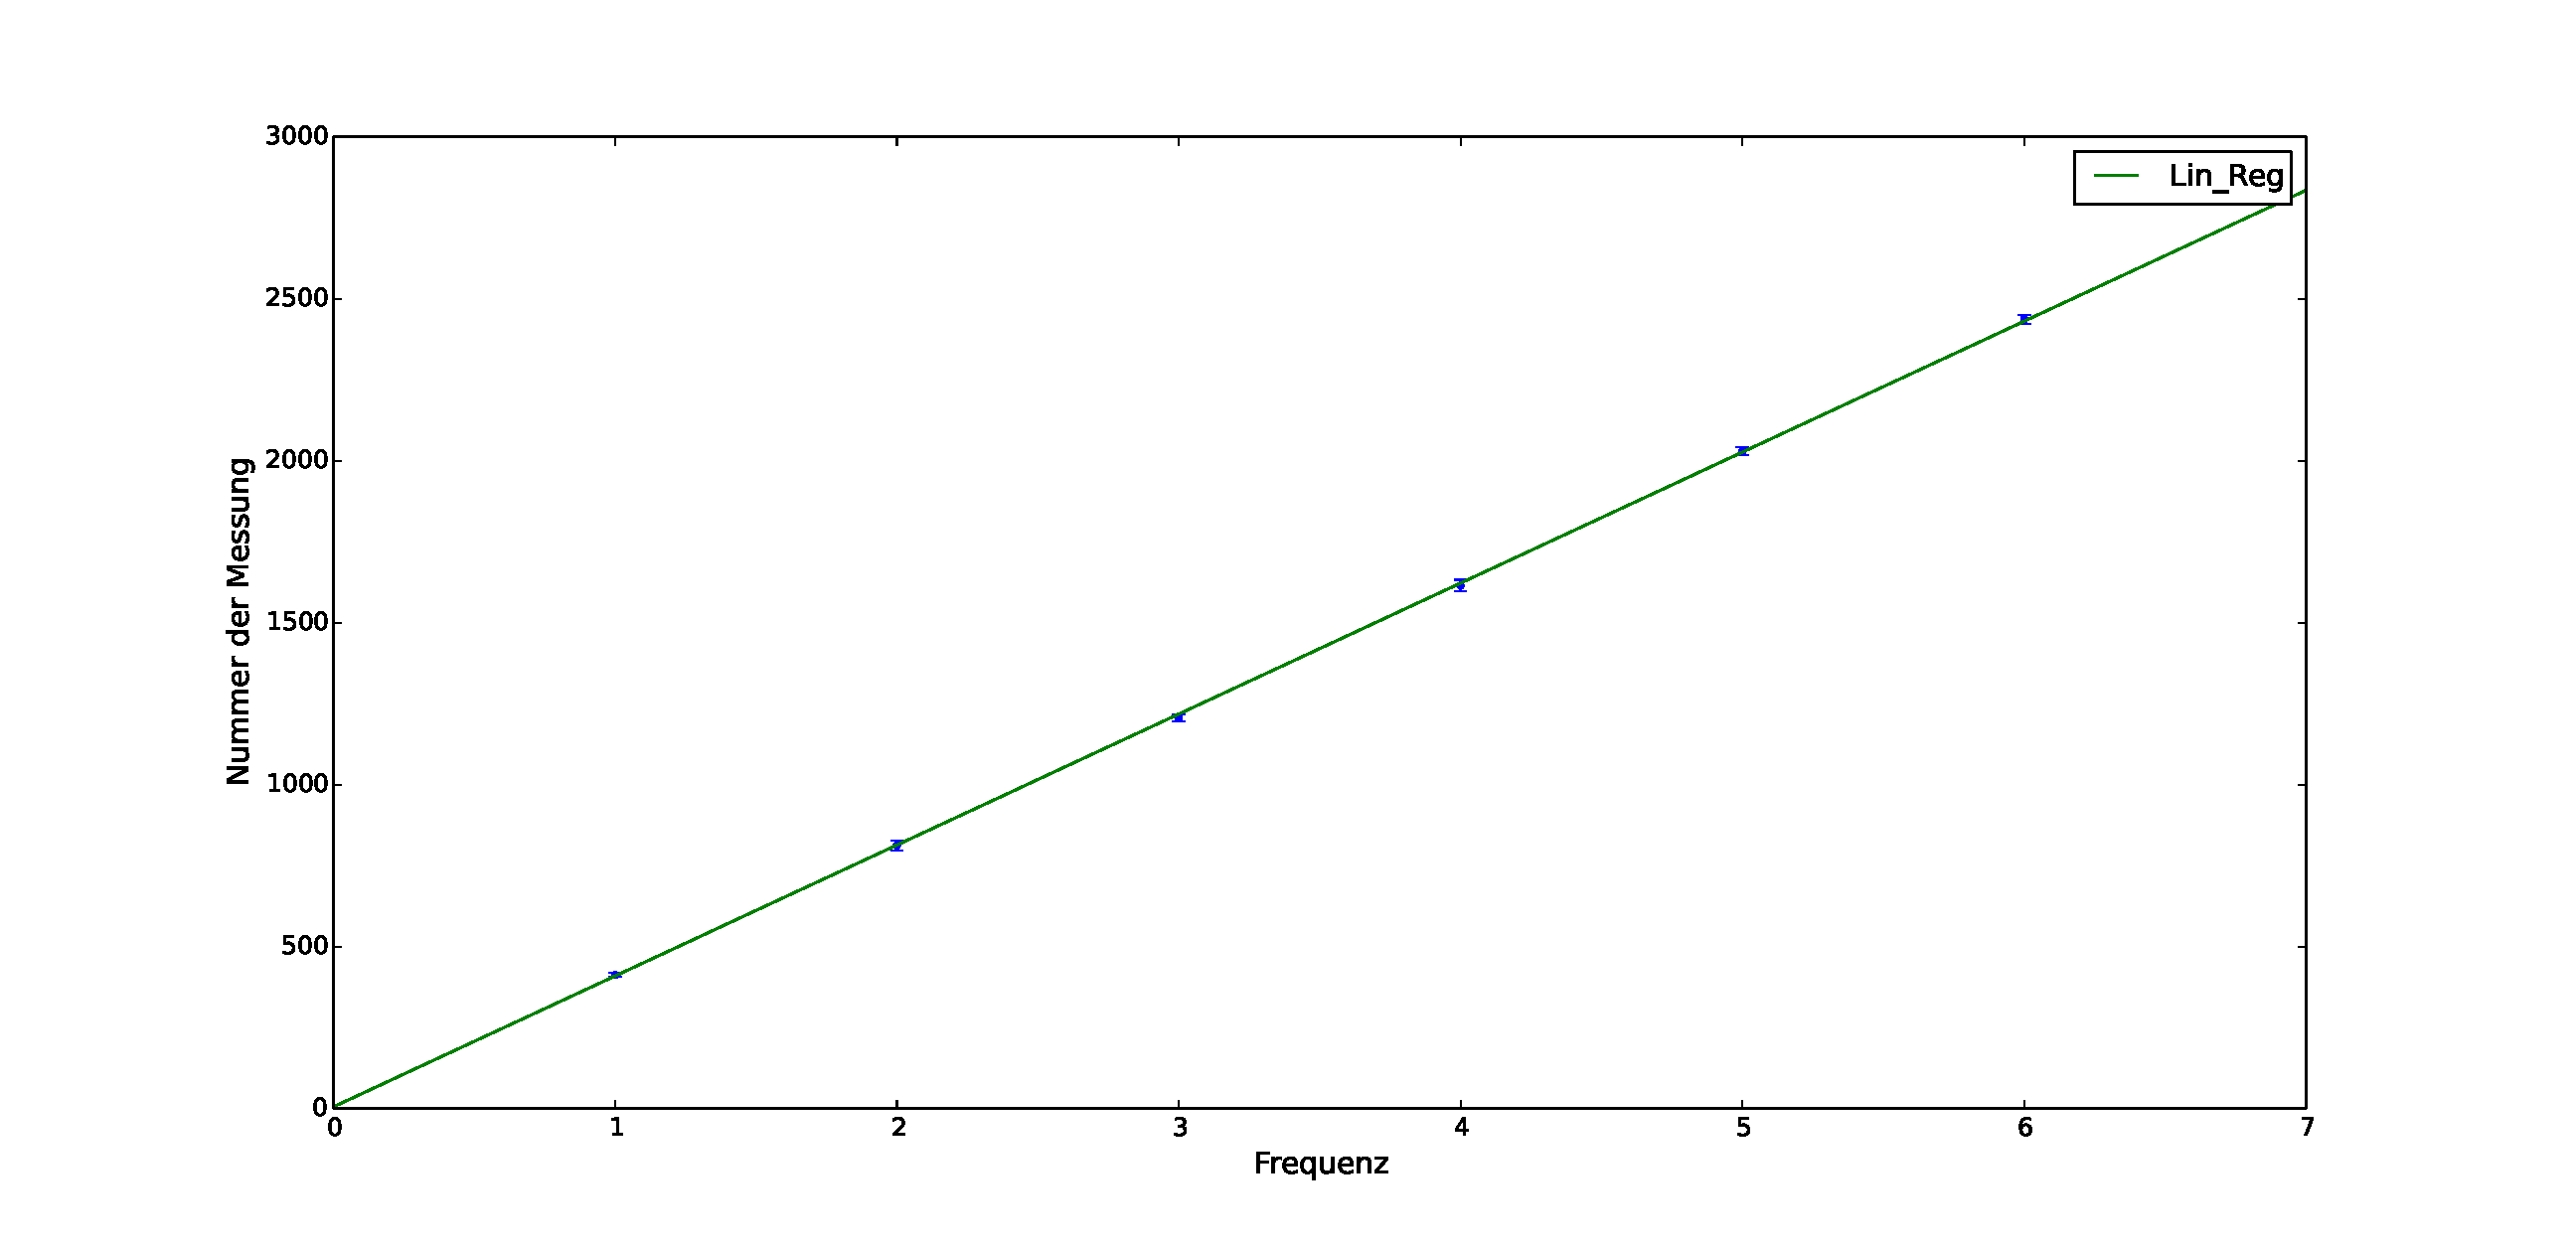
\includegraphics[scale=0.3]{Bilder/linreg_variation.eps}
\caption{Lineare Regression, die Steigung gibt $\frac{v_{Schall}}{2\cdot L}$ zurück}
\end{figure}
Mit einem $\chi^2 = 0.43$ ist unsere Anpassung in einem akzeptablen Rahmen. Das spiegelt sich auch in unserem Residuenplot wieder:
\begin{figure}[H]
\centering
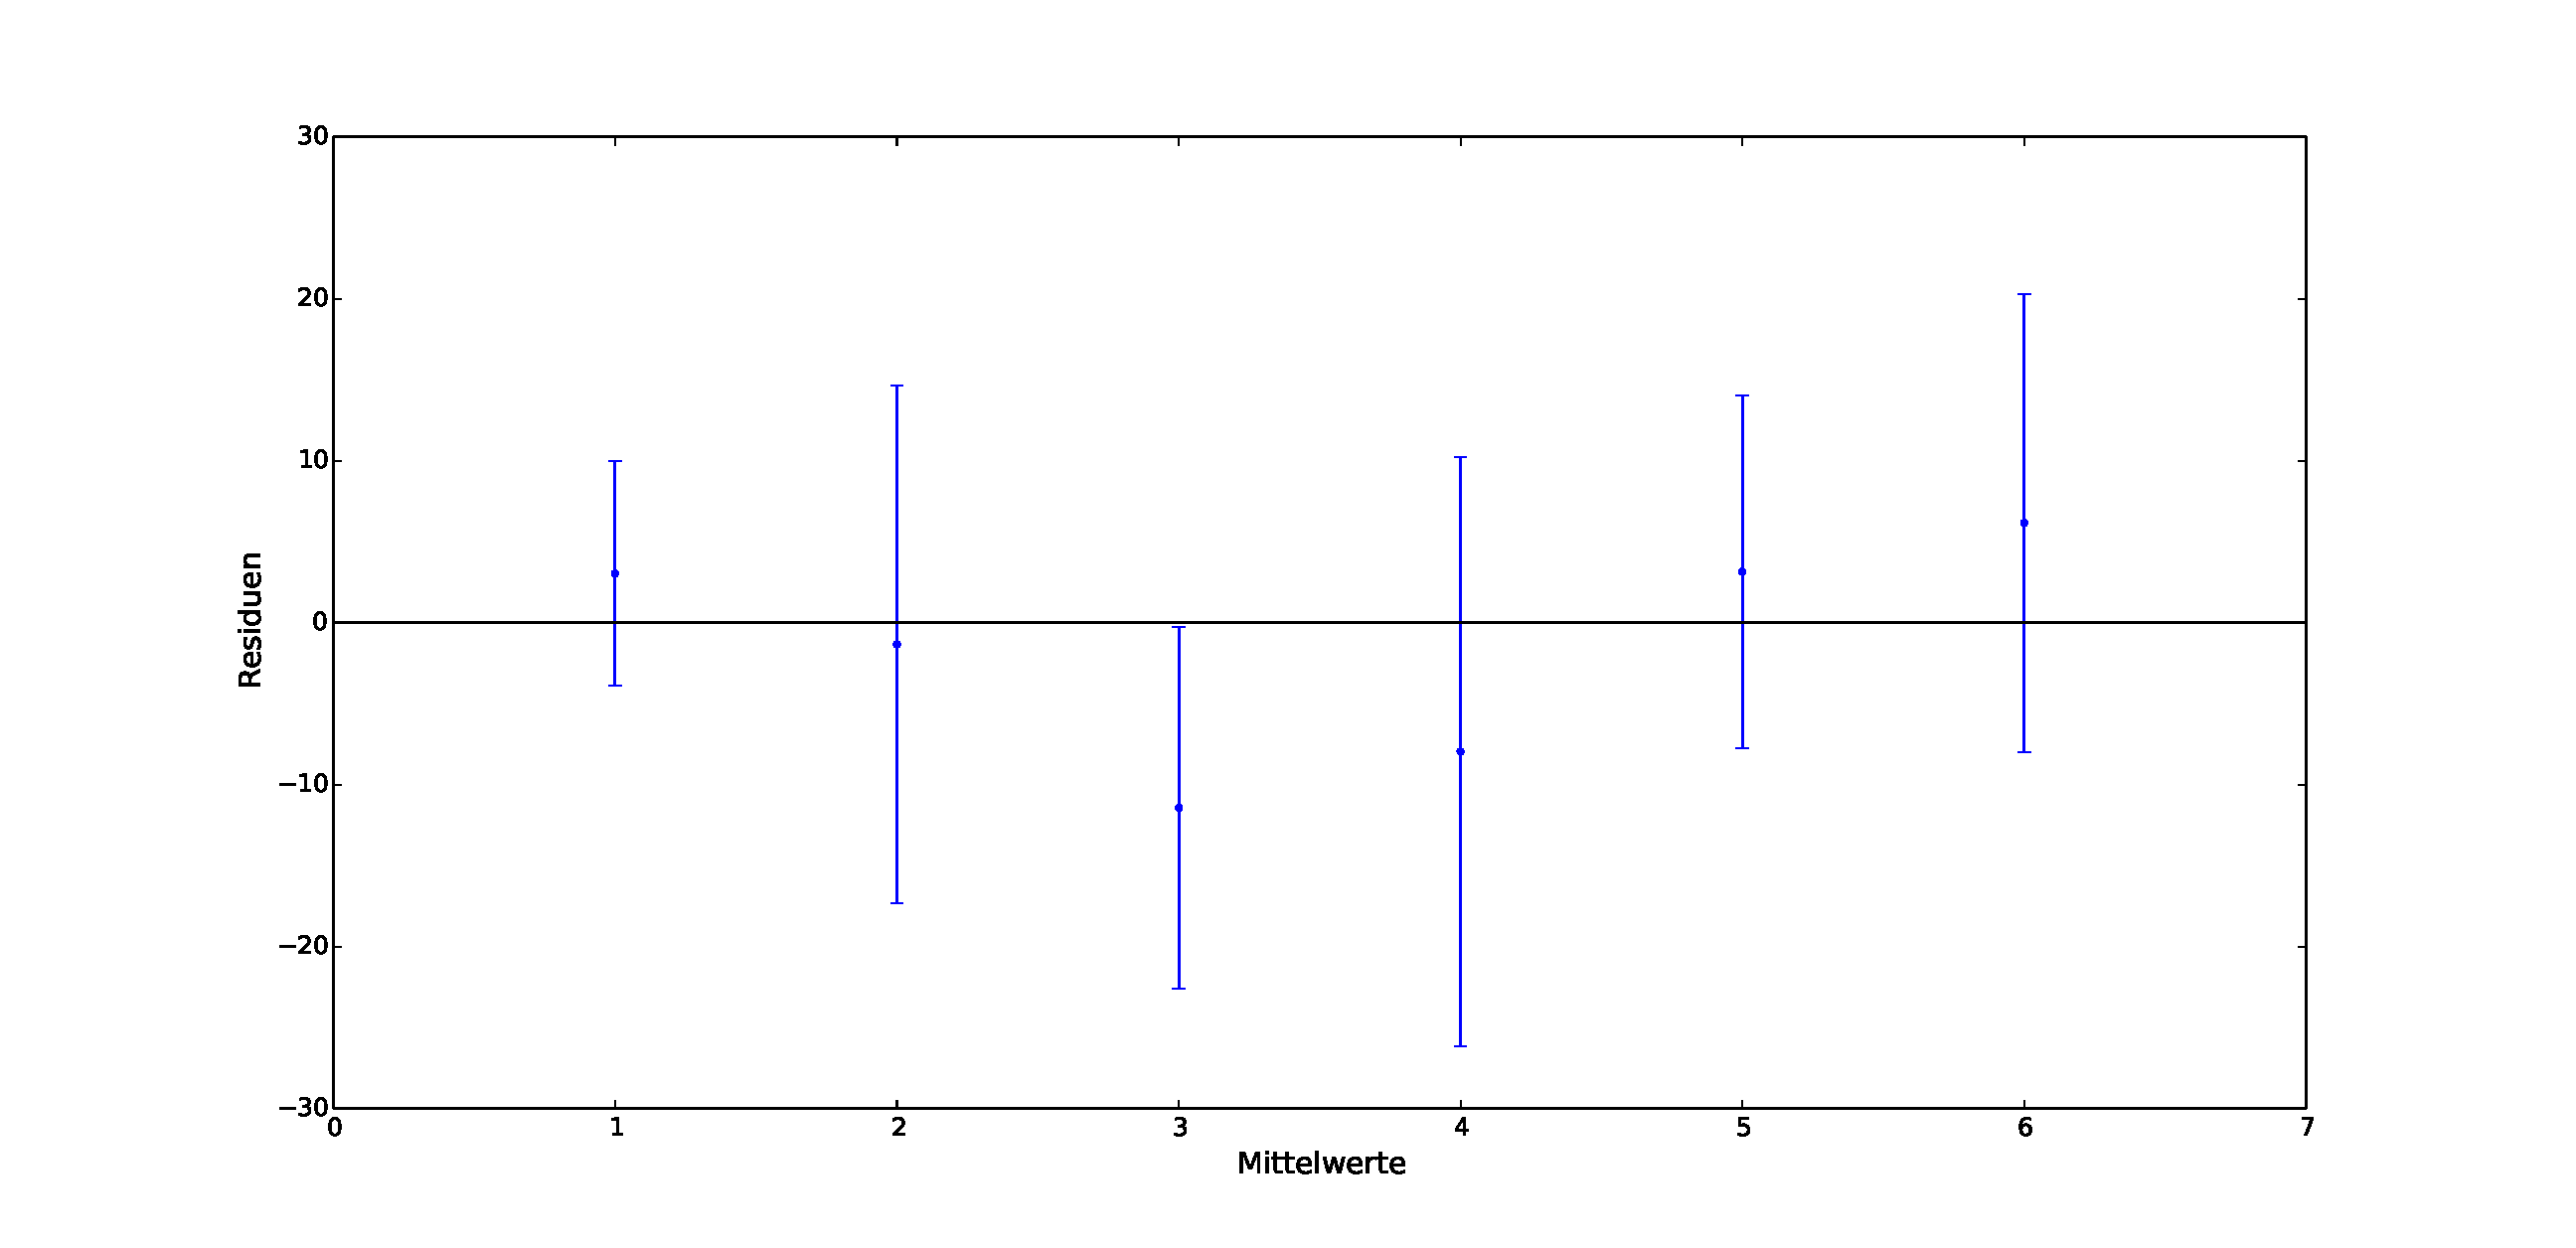
\includegraphics[scale=0.3]{Bilder/Residuen_Variation_Frequenzen.eps}
\caption{Residuenplot (Werte-Fit), zeigt Güte der Anpassung}
\end{figure}
Die Residuen streuen gleichverteilt um 0. 5 von 6 Werten schneiden die Nulllinie mit ihren Fehlerbalken, das entspricht $83.3\%$ der Werte die innerhalb von einem $\sigma$ den Sollwert schneiden. 
Die Steigung der Linearen Regression gibt uns die Schallgeschwindigkeit mit dem Faktor $\frac{1}{2\cdot L}$ wieder, wie auch schon in
\begin{equation}
f_n = \frac{n\cdot v}{2\cdot L}
\end{equation}
zu sehen ist.
Die Fehler auf die Längenmessung und die Fehler auf die Mittelwerte unserer Resonanzfrequenzen haben wir wie folgt fortgepflanzt:
\begin{equation}
\sigma_v = \sqrt{f_R^2\cdot\sigma_{\lambda}^2 + \lambda^2\cdot\sigma_f^2}
\end{equation}
mit
\begin{equation}
\sigma_{\lambda} = \sigma_{\bar{M}}\cdot\sqrt{2}
\end{equation}
$\bar{M}$ und $\sigma_{\bar{M}}$ haben wir erhalten durch:
\begin{equation}
\bar{M} = \frac{\sum_{i=1}^{N}{X_i}}{N}
\end{equation}
und
\begin{equation}
\sigma_{\bar{M}}=\frac{\sqrt{\frac{\sum_{i=1}^{N}({X_i-\bar{M}})^2}{N-1}}}{\sqrt{N}}
\end{equation}
Nach der Korrektur erhalten wir einen Wert für $v$ von
\begin{equation}
v = 343.46 \pm 2.08\,\frac{m}{s}
\end{equation}.

\subsection{Fazit}
Unser Wert für $v_{Schall}$ liegt innerhalb eines $\sigma$ Abstand zum Literaturwert (bei $T = 20^{\circ}\,$C) $v_{lit}=343\,\frac{m}{s}$. Unsere Fehlerabschätzungen führen zu einem relativen Fehler auf $v$ von $0.58\%$, was, zusammen mit unserem $\chi^2 = 0.43$ und Residuenplot, der keine Systematiken aufweist, sondern eine gleichverteilte Streuung um 0 zeigt, auf eine sehr präzise Messung schließen lässt, mit der wir als Gruppe zufrieden sind.

\end{document}